%  \documentclass[oneside,11pt]{article}

% 
\usepackage{soul}
\usepackage{natbib}
\usepackage{hyperref}
\usepackage{bookmark}
\usepackage{graphicx}             
\graphicspath{{./Figuras/}}

\usepackage{makecell}
\usepackage[margin=1in]{geometry}
\usepackage{float}                
\usepackage{amsmath}
\usepackage{amscd}
\usepackage{amsfonts}
\usepackage{amssymb}
\usepackage{bbm}
\usepackage{booktabs}
\usepackage{nameref}
\usepackage{multirow}
\usepackage[nokeyprefix]{refstyle}
\usepackage{rotating}
\usepackage{threeparttable}
\usepackage{afterpage}
\usepackage{lscape}
\usepackage{enumerate}
\usepackage{caption}
\usepackage{subcaption}
\usepackage{epstopdf}
\usepackage{setspace}
\usepackage{svg}
\usepackage{dsfont}
\usepackage{amsthm}
\usepackage{tocloft}
\usepackage{etoc}
\usepackage{lmodern}
\usepackage{bm}

\epstopdfDeclareGraphicsRule{.tiff}{png}{.png}{convert #1 \OutputFile}
\AppendGraphicsExtensions{.tiff}

\epstopdfDeclareGraphicsRule{.tif}{png}{.png}{convert #1 \OutputFile}
\AppendGraphicsExtensions{.tif}

\usepackage{tikz}
\usetikzlibrary{shapes.geometric, arrows}
\usetikzlibrary{calc}
\usetikzlibrary{matrix}

\tikzset{ 
    table/.style={
        matrix of nodes,
        row sep=-\pgflinewidth,
        column sep=-\pgflinewidth,
        nodes={
            rectangle,
            draw=black,
            align=center
        },
        minimum height=1.5em,
        text depth=0.5ex,
        text height=2ex,
        nodes in empty cells,
%%
        every even row/.style={
            nodes={fill=gray!20}
        },
        column 1/.style={
            nodes={text width=2em,font=\bfseries}
        },
        row 1/.style={
            nodes={
                fill=black,
                text=white,
                font=\bfseries
            }
        }
    }
}


\usepackage{colortbl}

\newtheorem{theorem}{Theorem}
\newtheorem{claim}[theorem]{Claim}
\newtheorem{prop}[theorem]{Proposition} 
\newtheorem{cor}[theorem]{Corollary} 

\DeclareRobustCommand{\hlgr}[1]{{\sethlcolor{green}\hl{#1}}}


\usepackage{comment}
%para esconder columnas en tablas (enrique)
\usepackage{array}
\newcolumntype{H}{>{\setbox0=\hbox\bgroup}c<{\egroup}@{}}
\linespread{1.25}

\newcommand{\wh}{\widehat}
\usepackage{anyfontsize}

\usepackage[linesnumbered,vlined,ruled,commentsnumbered]{algorithm2e}

\DontPrintSemicolon
\newcommand{\To}{\mbox{\upshape\bfseries to}}
% %%% HELPER CODE FOR DEALING WITH EXTERNAL REFERENCES
% \usepackage{xr}
% \makeatletter
% \newcommand*{\addFileDependency}[1]{
%   \typeout{(#1)}
%   \@addtofilelist{#1}
%   \IfFileExists{#1}{}{\typeout{No file #1.}}
% }
% \makeatother


% \newcommand*{\myexternaldocument}[1]{
%     \externaldocument{#1}
%     \addFileDependency{#1.tex}
%     \addFileDependency{#1.aux}
% }

% %\myexternaldocument{OA}

% %%%%%%%%%%%%%%%%%%%%%%%%%%%%%%%% DOCUMENT
% \begin{document}

%%%%%%%%%%%%%%%%%%%%%%%%%%%%%%%%%%%%%%%%%%%%%%%

% APPENDIX 
\setcounter{table}{0}
\setcounter{figure}{0}
\setcounter{section}{0}
\pagenumbering{gobble}


\begin{center}
	\LARGE The limits of self-commitment and private paternalism \\[0.5em]
	\Large{Appendix $-$ For Online Publication} \\[1em]
	\large \author{Craig McIntosh \and Isaac Meza \and Joyce Sadka \and Enrique Seira}
\end{center}

\appendix
\pagenumbering{arabic}
\renewcommand\thefigure{OA-\arabic{figure}}
\renewcommand\thetable{OA-\arabic{table}}
\renewcommand*{\thepage}{OA - \arabic{page}}
\renewcommand\thesection{Appendix \Alph{section}.}
\renewcommand\thesubsection{\Alph{section}.\arabic{subsection}}

%\renewcommand{\cftparskip}{0em} % NOT NEEDED
\renewcommand\cftsecdotsep{\cftdotsep}
\renewcommand\cftsubsecdotsep{\cftnodots}
\renewcommand{\cftsecnumwidth}{6em}
 \renewcommand{\cftpnumalign}{r}
%\renewcommand{\cftsecleader}{\normalfont\cftdotfill{\cftsecdotsep}}


\renewcommand{\cftsecleader}{\cftdotfill{\cftsecdotsep}\hspace{1.8em}}
%\renewcommand{\cftsecpagefont}{20em}
%\renewcommand{\cftfignumwidth}{6em}
%\renewcommand{\cfttabnumwidth}{3.3em}

%\tableofcontents
\etocdepthtag.toc{mtappendix}
\etocsettagdepth{mtchapter}{none}
\etocsettagdepth{mtappendix}{subsection}

\setstretch{0.9}
%\renewcommand\contentsname{} % the empty name

\begingroup
\let\clearpage\relax
%\vspace{-1.5em} % the removed space. Set as appropriate
\tableofcontents
\endgroup


\newpage



\section{ }
\vspace{.2in}




\vspace{.1in}


\begin{figure}[H]
     \caption{Some Pawnshops}
    \label{PawnshopPicture}
    \begin{center}
    \begin{subfigure}{0.42\textwidth}
    \caption{Appraiser/tellers inside a pawnshop}
        \centering
        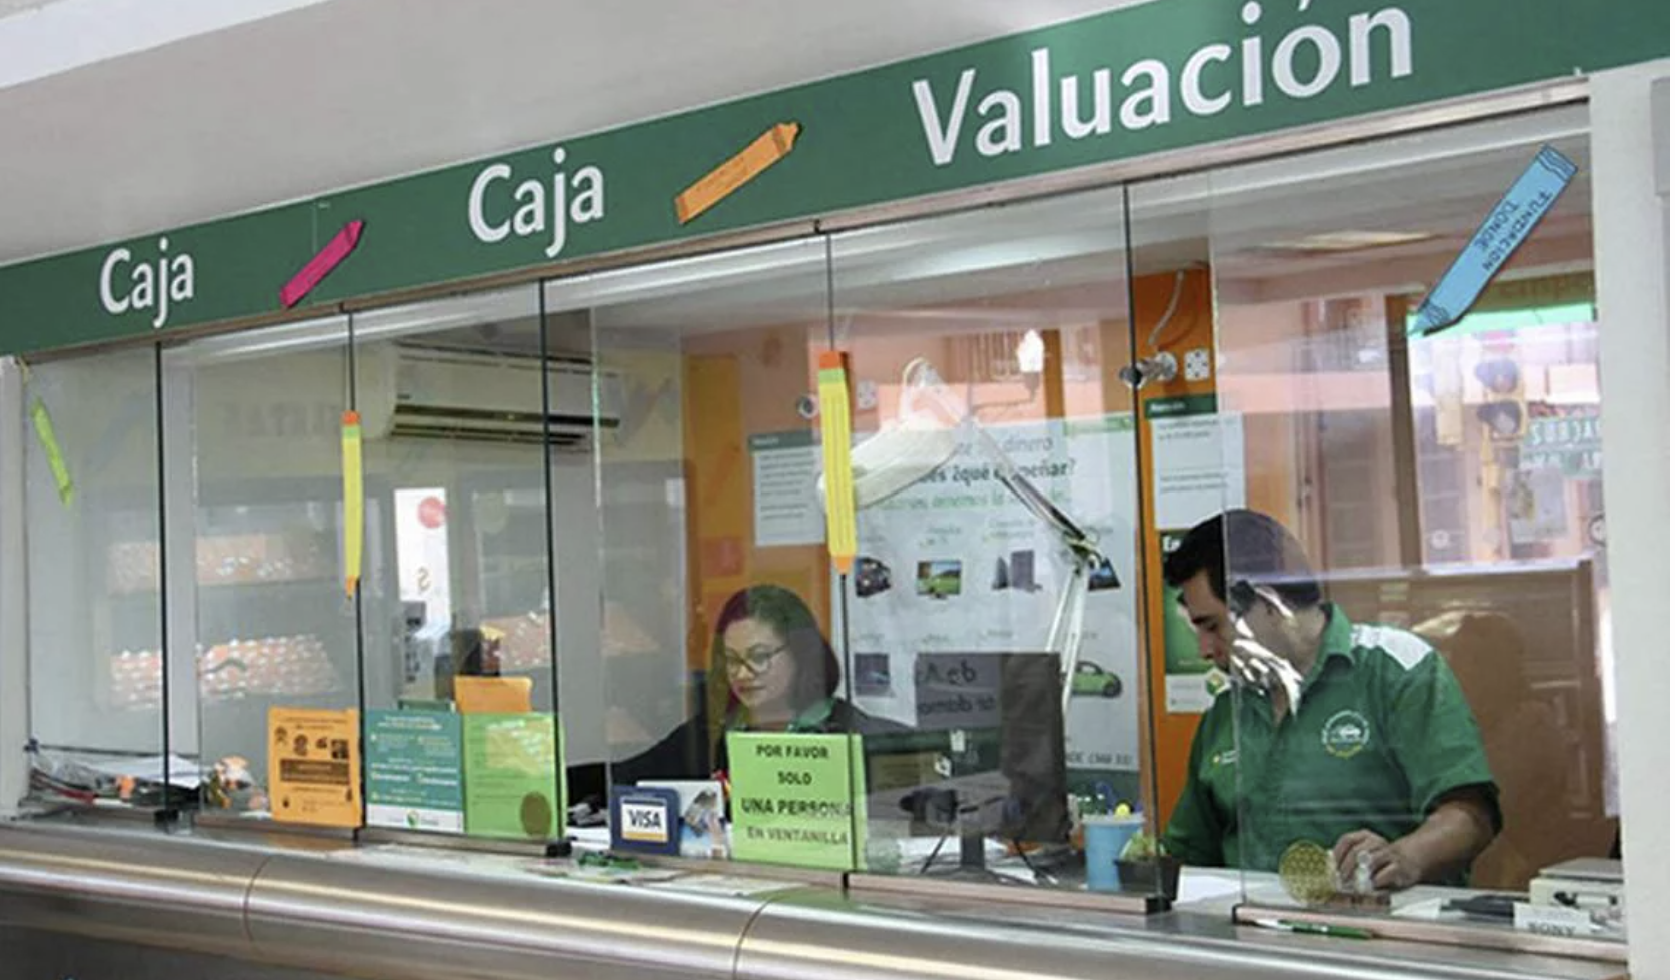
\includegraphics[width=\textwidth]{Figuras/empenio9.png}
    \end{subfigure}
        \begin{subfigure}{0.45\textwidth}
    \caption{Pawnshop}
        \centering
        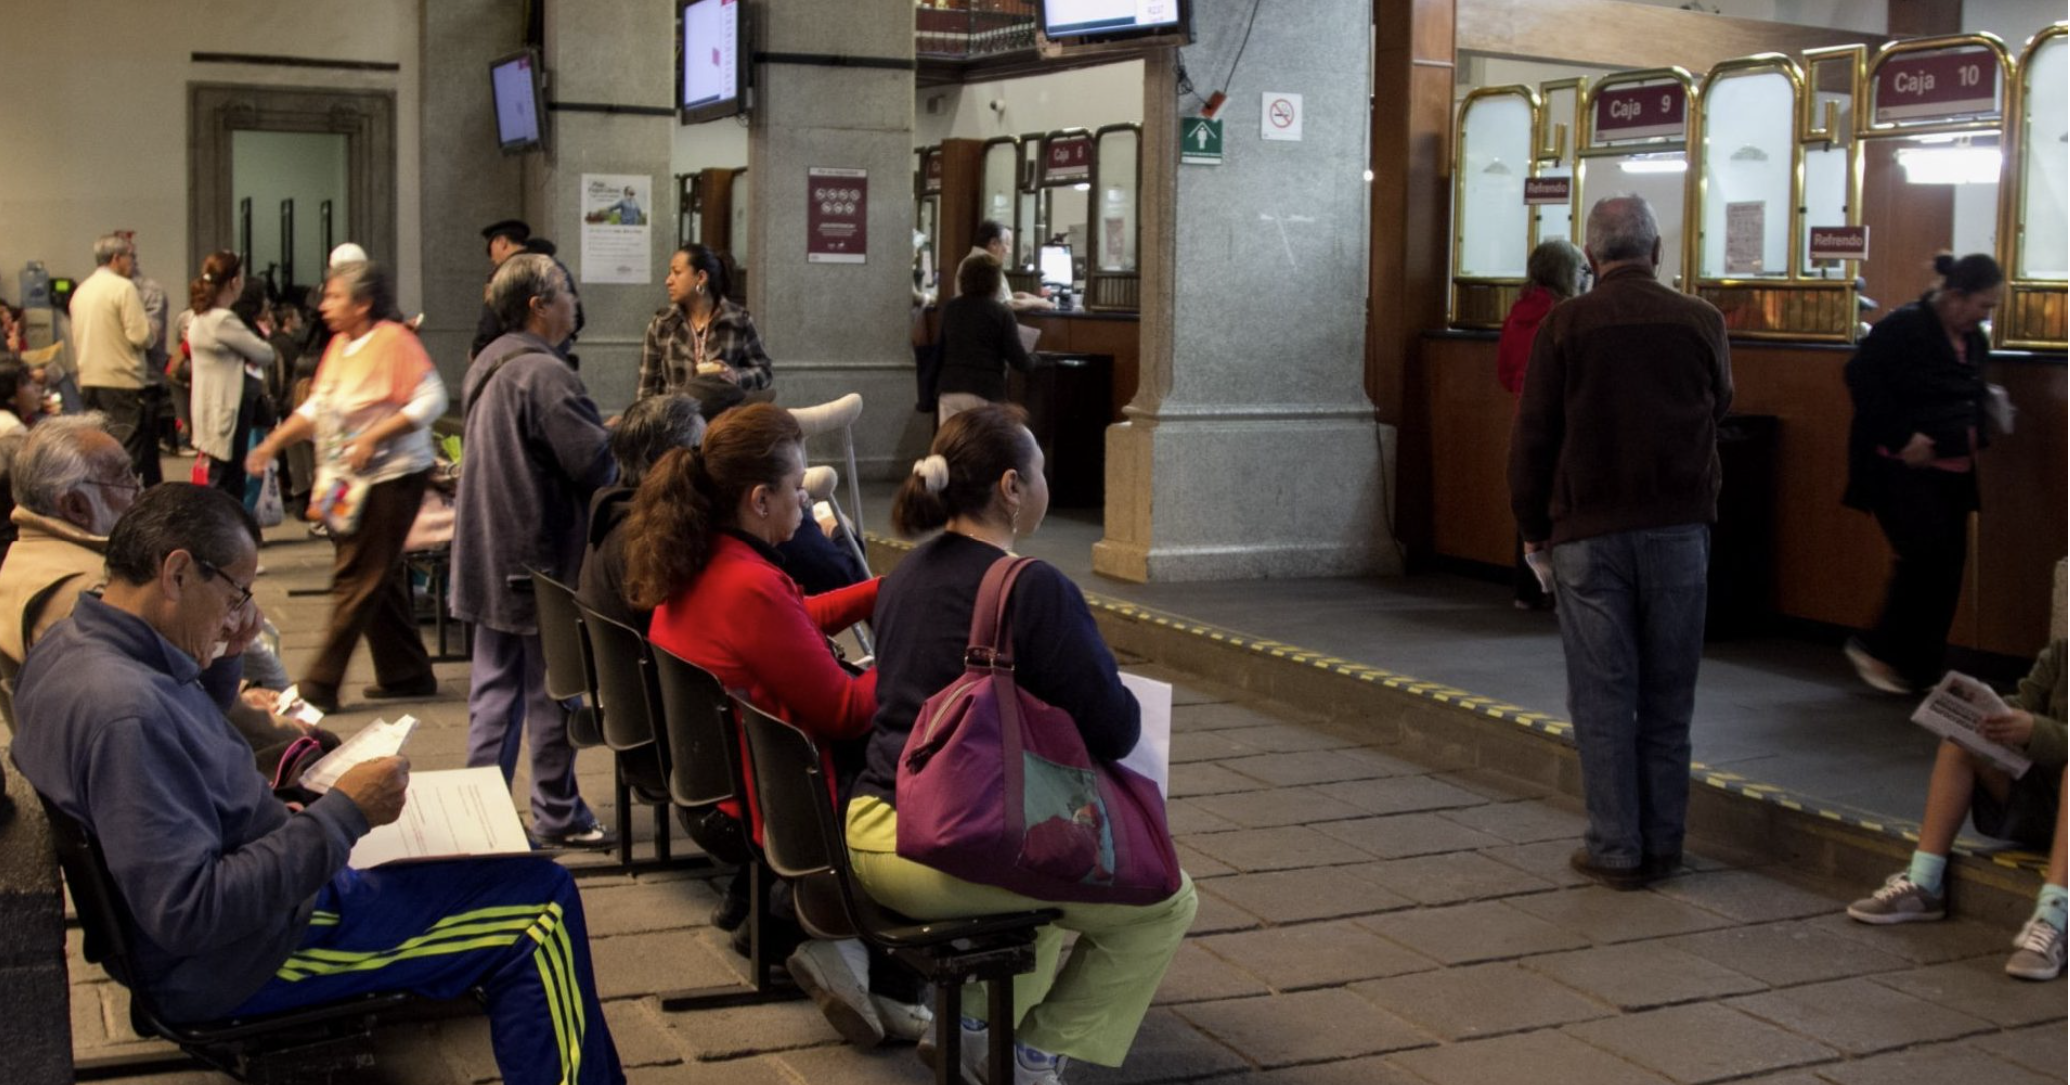
\includegraphics[width=\textwidth]{Figuras/empenio11.png}
    \end{subfigure}
    
        \vspace{3ex}

    \begin{subfigure}{0.45\textwidth}
    \caption{Pawnshop}
        \centering
        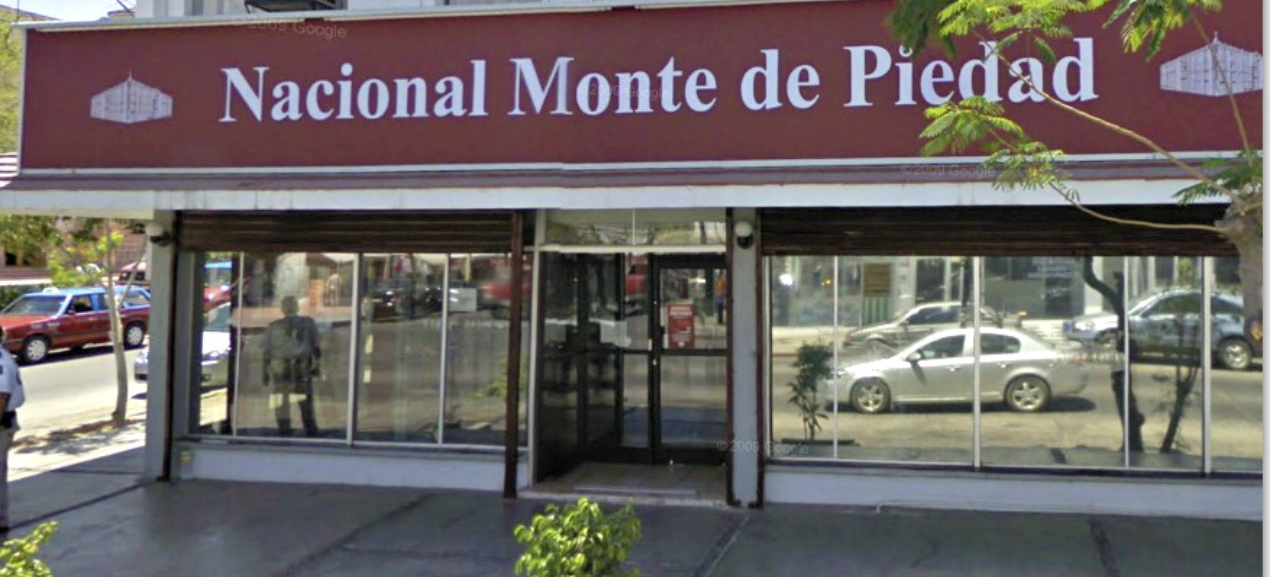
\includegraphics[width=\textwidth]{Figuras/empenio2.png}
    \end{subfigure}
    \begin{subfigure}{0.42\textwidth}
    \caption{Lost pawns which are for sale}
        \centering
        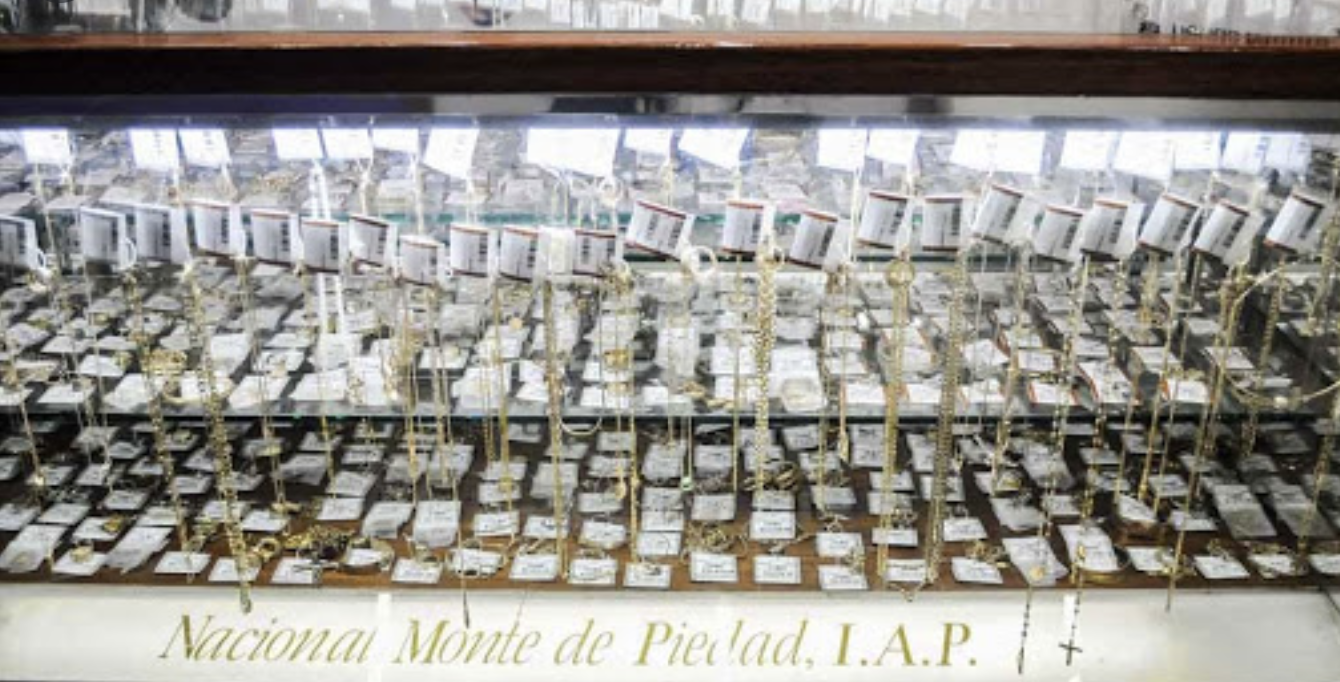
\includegraphics[width=\textwidth]{Figuras/empenio3.png}
    \end{subfigure}
    \end{center}
    \scriptsize
        This figure  shows pictures of pawnshops in Mexico city. They do not necessarily coincide with Lender P for confidentiality. 
\end{figure}



\vspace{.1in}
\begin{figure}[H]
     \caption{Gold buyers next to pawnshops}
    \label{GoldBuyers}
    \begin{center}
    \begin{subfigure}{.49\textwidth}
    \caption{Gold buyer next to pawnshop 1}
        \centering
        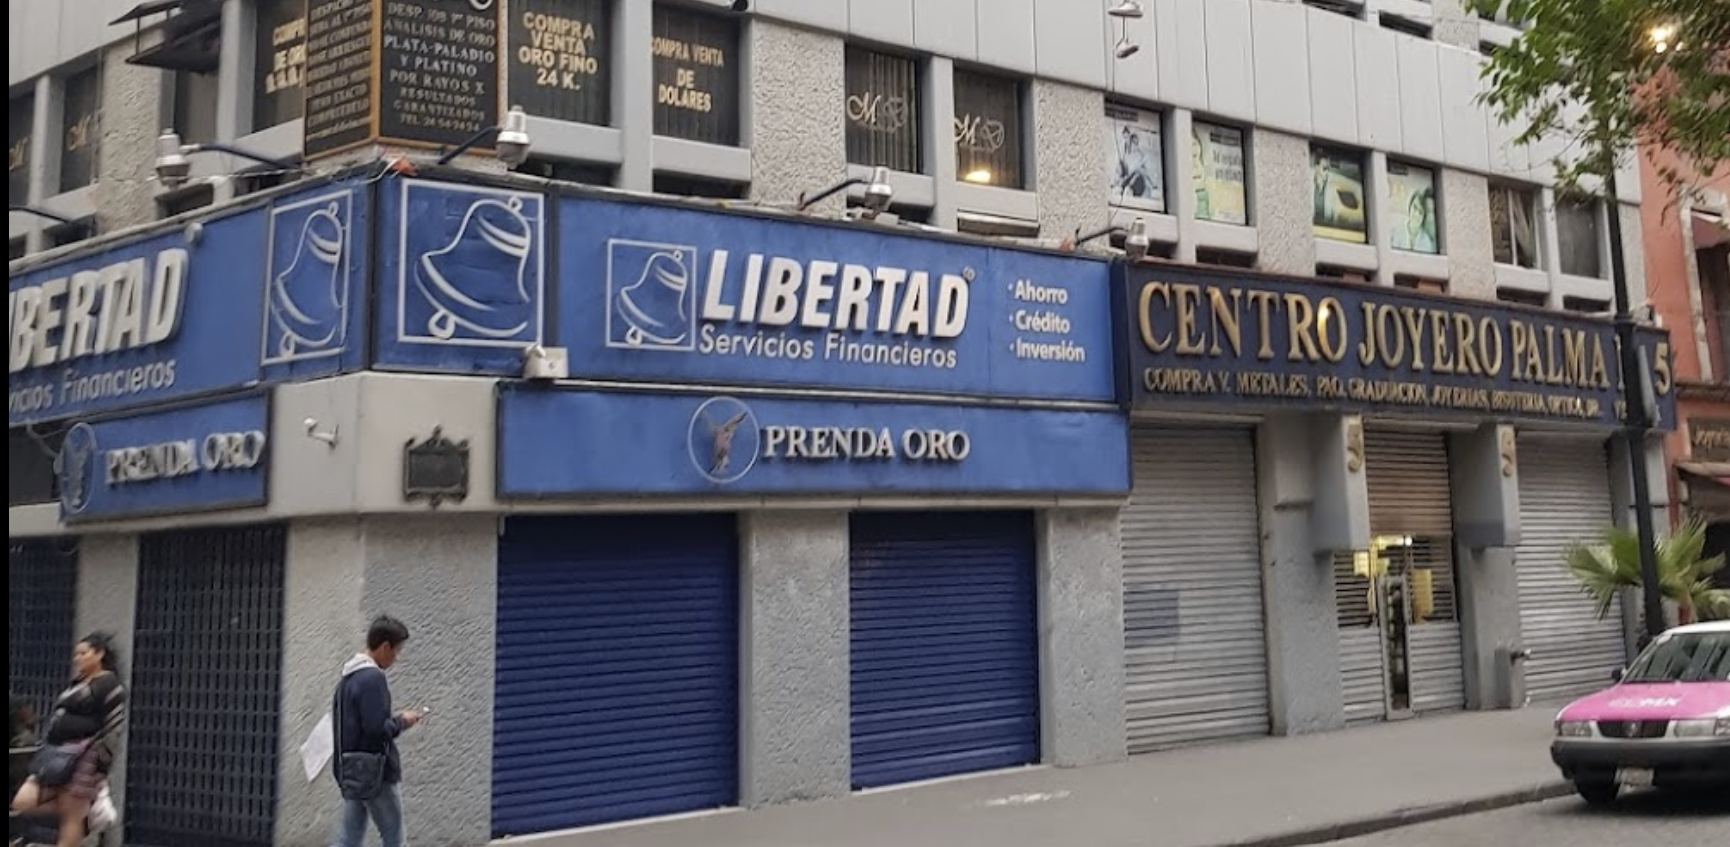
\includegraphics[width=\textwidth]{Figuras/empenio7.png}
    \end{subfigure}
    \begin{subfigure}{.49\textwidth}
    \caption{Gold buyer next to pawnshop 1}
        \centering
        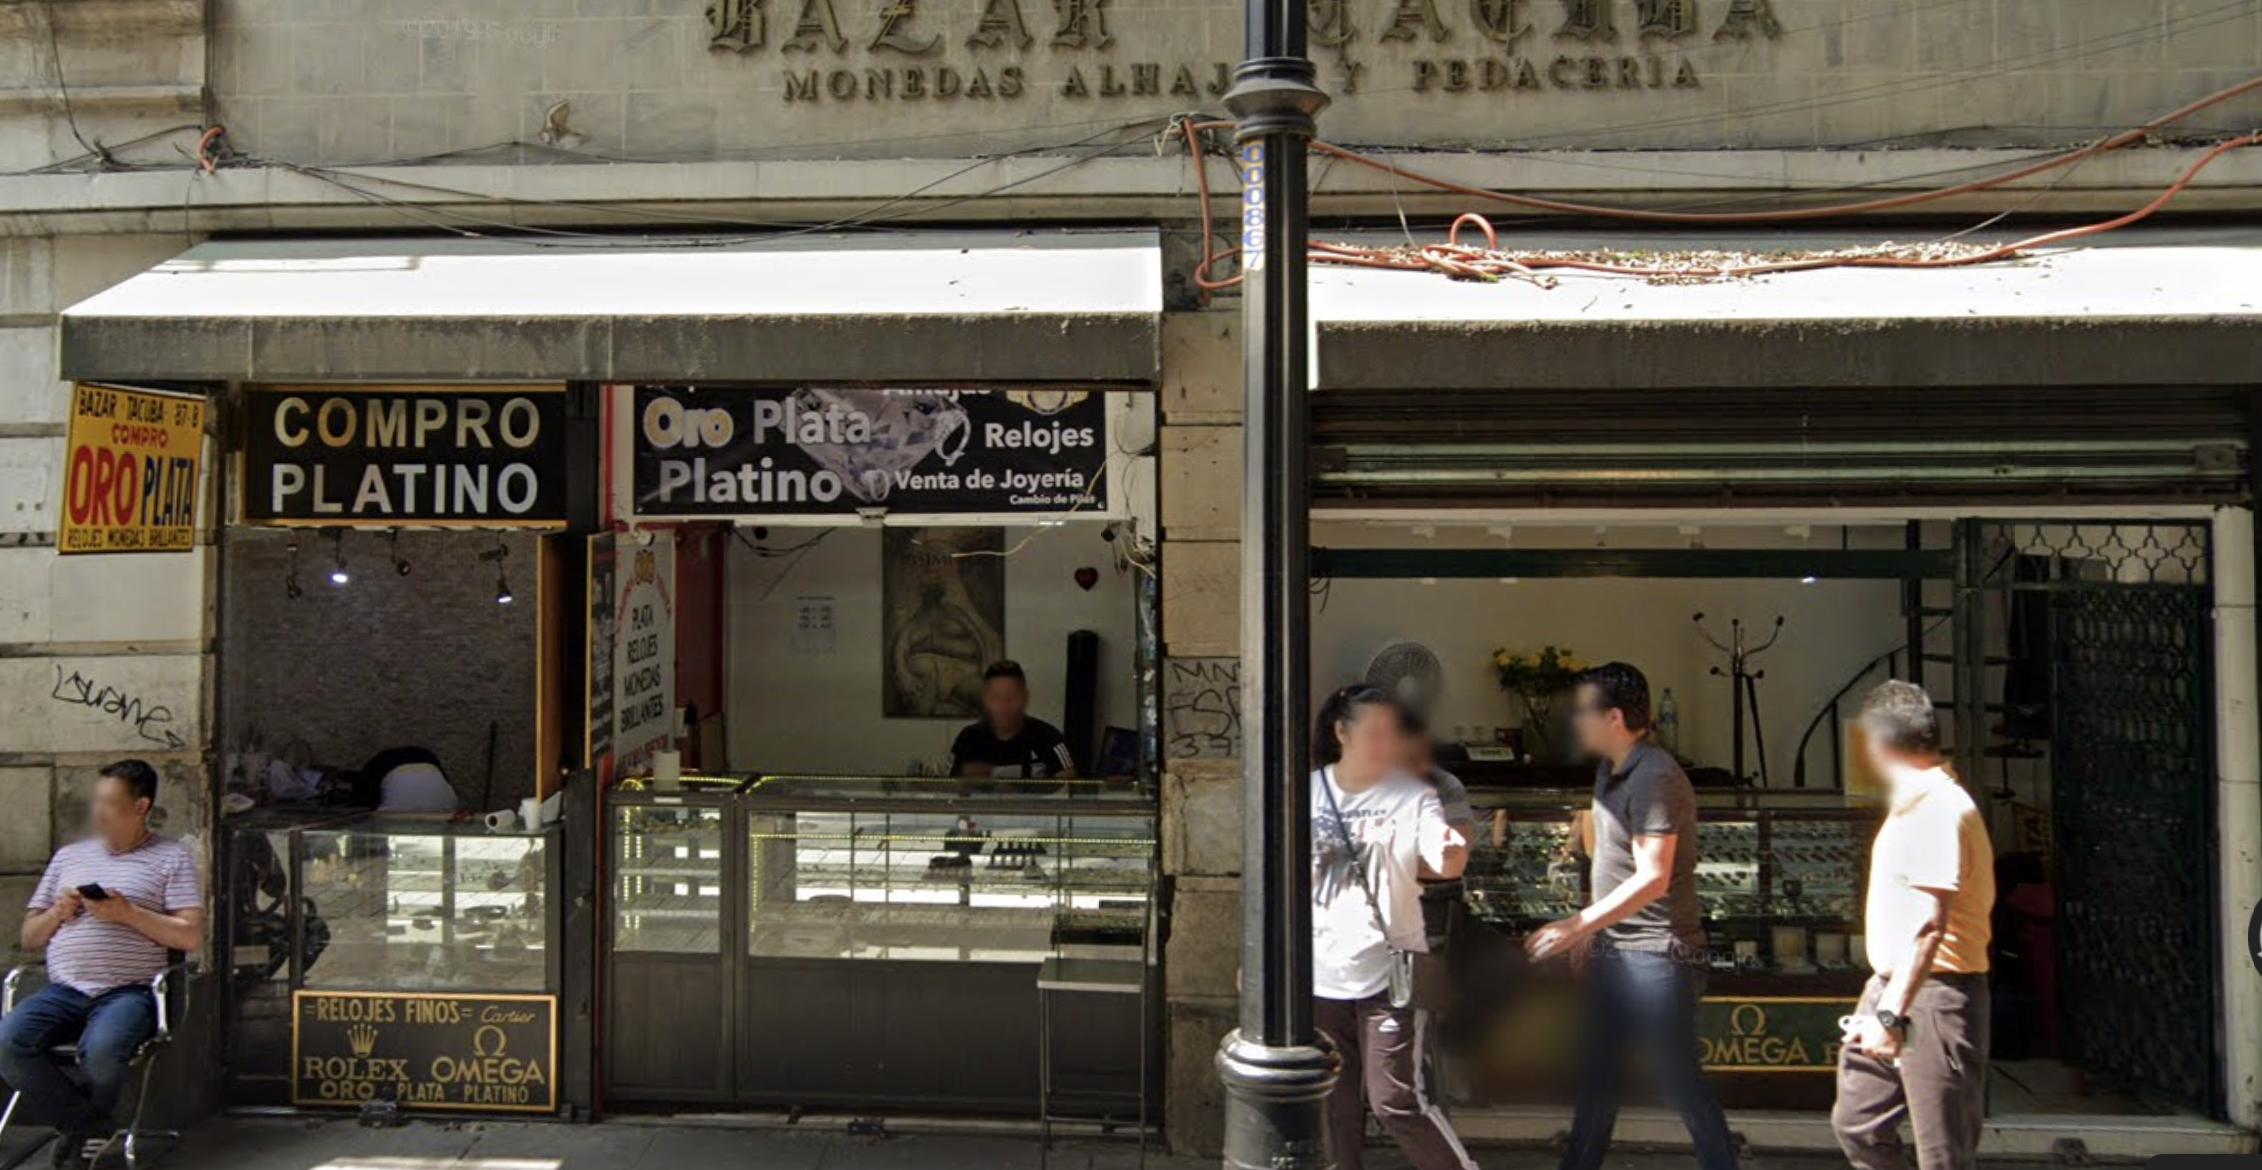
\includegraphics[width=\textwidth]{Figuras/empenio8.png}
    \end{subfigure}
       \vspace{3ex}
       
    \end{center}
    \scriptsize
        This figure shows pictures of gold buyers next to pawnshops in Mexico city. They do not necessarily coincide with Lender P for confidentiality. 
\end{figure}




\begin{table}[H]
\caption{Number of pawns balance before and after the experiment}
\label{num_pawns_bal}
\begin{center}
\scriptsize{% Table generated by Excel2LaTeX from sheet 'num_pawns_bal'
\begin{tabular}{lcccc}
\toprule
      & \multicolumn{4}{c}{Pawns per day} \\
\midrule
      & 0-degree & 1-degree & 2-degree & 3-degree \\
\midrule
\midrule
      & (1)   & (2)   & (3)   & (4) \\
\midrule
\midrule
$\beta_a$ & 2.48  & -3.32 & -0.65 & -0.65 \\
      & (1.36) & (1.85) & (2.80) & (2.80) \\
$\beta_b$ & 0.20  & 1.82  & 1.32  & 1.32 \\
      & (0.97) & (0.93) & (0.67) & (0.67) \\
      &       &       &       &  \\
\midrule
Observations & 628   & 628   & 628   & 628 \\
R-sq  & 0.737 & 0.747 & 0.747 & 0.747 \\
Branch FE & \checkmark & \checkmark & \checkmark & \checkmark \\
\bottomrule
\bottomrule
\end{tabular}%
}
\end{center}
 \scriptsize 
%\textit{Do file: } \texttt{num\_pawns\_bal.do}
\end{table}



\subsection{Surveys}

\afterpage{
\begin{table}[H]
\caption{Baseline survey}
\label{baseline_survey}
\begin{center}
\scriptsize{% Table generated by Excel2LaTeX from sheet 'transcribed'
\begin{tabular}{cl}
\toprule
      & \textbf{Baseline Survey} \\
\midrule
\midrule
1     & \textbf{Your pawn was:} \\
      & (a) Inherite, (b) a gift, (c) bought by me, (d) lend to me, (e) other \_\_\_\_\_\_\_\_\_\_\_\_ \\
2     & \textbf{Mark with an "X" in the line below how likely is that you recover your pawn. } \\
      & \textbf{Where 0 is impossible and 100 is completely certain} \\
3     & \textbf{How much do you think the item you plan to pawn is worth?       \_\_\_\_\_\_\_\_\_\_\_\_\_\_ pesos} \\
4     & \textbf{Gender      } \\
5     & \textbf{Age} \\
6     & \textbf{Civil Status } \\
      & (a) married, (b) single, (c) divorced, (d) widowed \\
7     & \textbf{Work status} \\
      & (a) employed, (b) own business, (c) houseshores, (d) don't work, (e) retired, (f) study \\
8     & \textbf{Education} \\
      & (a) no formal education, (b) primary, (c) middle school, (d) highschool, (e) more than highschool \\
9     & \textbf{In the last month, did a friend or family member asked you for money?} \\
      & (a) yes  (b) no \\
10    & \textbf{What would you like to have: 100 pesos tomorrow or 150 pesos in one month?} \\
11    & \textbf{How often do you feel stressed by your economic situation?} \\
      & (a) always, (b) very often, (c) sometimes, (d) never \\
12    & \textbf{What is the main reason you want to pawn?} \\
      & (a) Need the money because somebody in my family lost his/her job \\
      & (b) Need the money to pay for a sickness in the family \\
      & (c) Need the money for an urgent expense \\
      & (d) Need the money for some non urgent expense. \\
13    & \textbf{How stressed do you feel from the situation that led to to pawn?} \\
      & (a) very stressed, (b) somwhat stressed, (c) a little stressed, (d) not stressed  \\
14    & \textbf{In 3 months, I expect to have a  \_\_\_\_\_\_\_\_\_\_\_\_\_\_\_\_ situation} \\
      & (a) better, (b) similar,  (c) worse \\
15    & \textbf{Have you panwned before?} \\
      & (a) yes  (b) no \\
16    & \textbf{How many times have you pawned on a Lender P branch?} \\
      & (a) NO\_\_\_    (b)  1-2 times \_\_\_    (c) 3-5 times\_\_\_\_   (d) More than 5\_\_\_\_ \\
17    & \multicolumn{1}{p{54.91em}}{\textbf{If you are saving money and a family member wants to use it for something }} \\
      & \multicolumn{1}{p{54.91em}}{(a) I would only give him the money for an urgent expenze} \\
      & \multicolumn{1}{p{54.91em}}{(b) I would give him the money even if it was not an urgent expense} \\
      & \multicolumn{1}{p{54.91em}}{(c) I would not give him/her the money regardless} \\
      & \multicolumn{1}{p{54.91em}}{(d) No one would ask me for my money} \\
18    & \textbf{Do you make an expenses budget for the month ahead of time?} \\
      & (a) always, (b) very often, (c) sometimes, (d) never \\
19    & \multicolumn{1}{p{54.91em}}{\textbf{Do you have other items you could pawn?}} \\
      & (a) yes  (b) no \\
20    & \textbf{Do you have savings?} \\
      & (a) yes  (b) no \\
21    & \textbf{Do you participate in a ROSCA?} \\
      & (a) yes  (b) no \\
22    & \textbf{Is it common that family or friends ask for money?} \\
      & (a) yes  (b) no \\
23    & \textbf{How much did you spend to come to the branch today?    \$\_\_\_\_\_\_\_\_\_\_\_\_\_\_ pesos} \\
24    & \textbf{How much time does it usually take to come to this branch?    \_\_\_\_\_\_\_\_\_\_\_} \\
25    & \textbf{How much does your family spend in a normal week?   \$\_\_\_\_\_\_\_\_\_\_\_\_\_\_ pesos} \\
26    & \textbf{How much do you manage to save in a normal week?   \$\_\_\_\_\_\_\_\_\_\_\_\_\_\_ pesos} \\
27    & \textbf{Does it happen to you that you spend more than you wanted because you fall into temptation?} \\
      & (a) never, (b) almost never, (c) sometimes, (d) very often \\
28    & \textbf{In the last 6 months, has it happened that at some point you lacked money to pay} \\
      & (a) rent?    (b) food    (c)food   (d) medicine  (e) electricity   (f) heating   (g) telephone    (i) water \\
29    & \textbf{What would you like to have: 100 pesos in 3 months or 150 pesos in four months?} \\
30    & \textbf{Would you like to receive (free) reminders for upcomming payments?} \\
      & (a) yes  (b) no \\
\bottomrule
\end{tabular}%
}
\end{center}
\end{table}
}



\newpage
\subsection{Some more evidence of overconfidence}

\vspace{.2in}
\begin{figure}[H]
    \caption{Behavior of those who lost pawn}
    \label{proxy_naive}
    \begin{center}
    \begin{subfigure}{0.40\textwidth}
        \caption{Elapsed days to first payment}
        \centering
        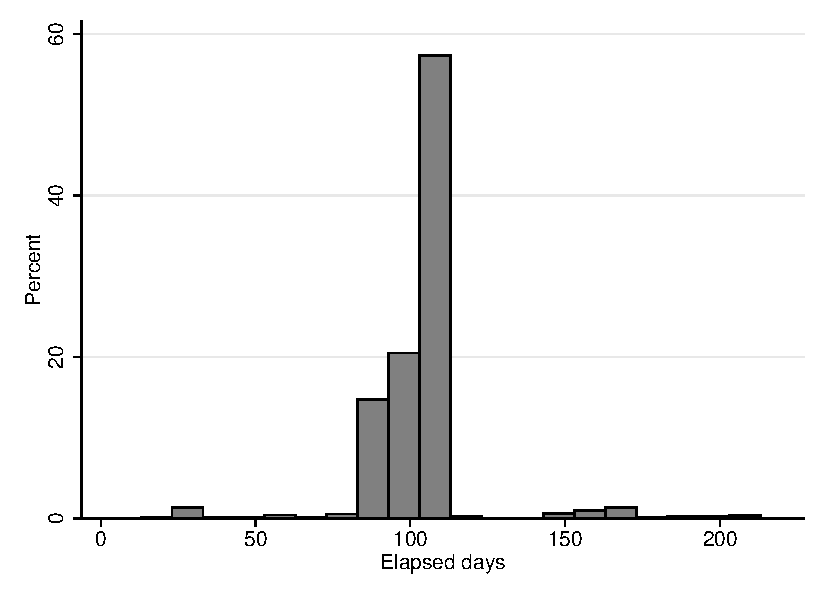
\includegraphics[width=\textwidth]{Figuras/hist_firstdays_default.pdf}
    \end{subfigure}
    \begin{subfigure}{0.40\textwidth}
        \caption{Elapsed days to last payment}
        \centering
        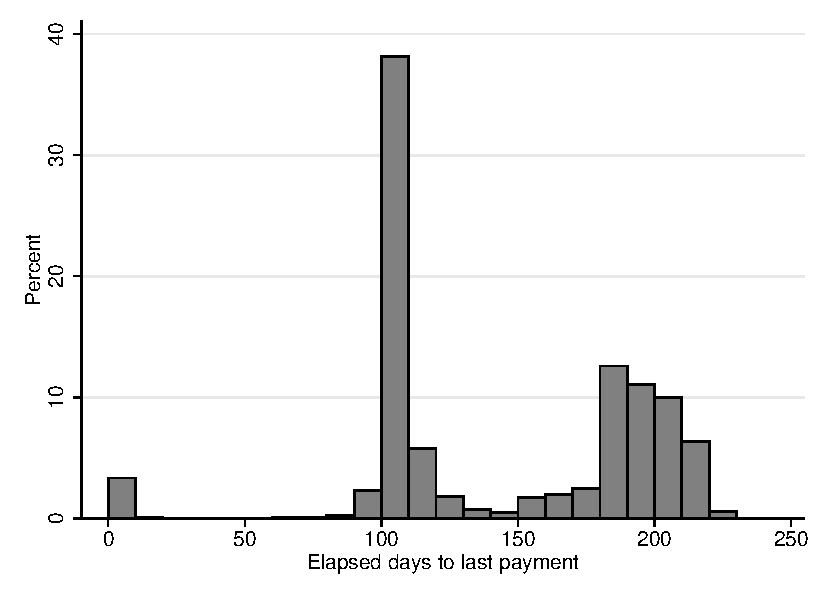
\includegraphics[width=\textwidth]{Figuras/hist_days_default.pdf}
    \end{subfigure}
        \begin{subfigure}{0.40\textwidth}
        \caption{Payments as \% of loan}
        \centering
        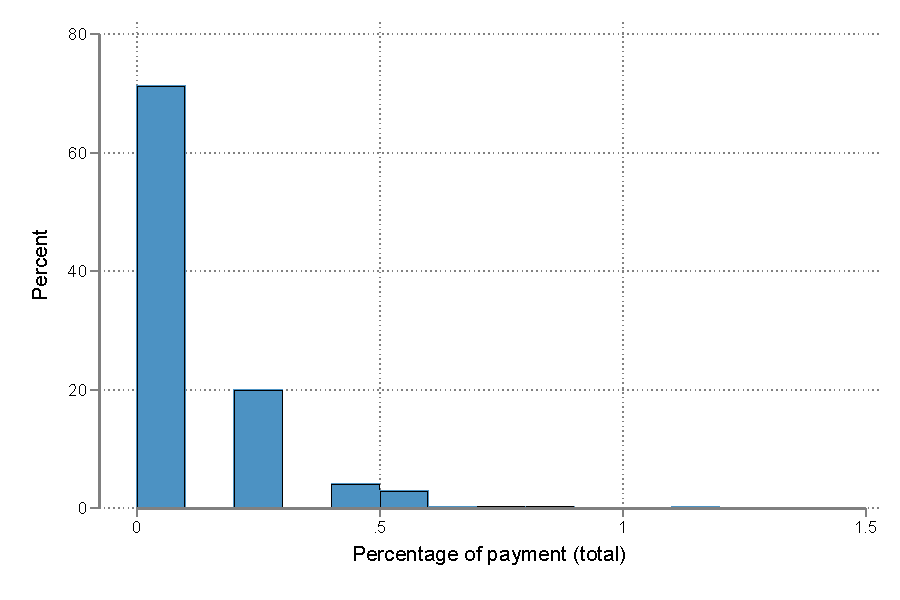
\includegraphics[width=\textwidth]{Figuras/hist_percpay_default.pdf}
    \end{subfigure}
    \begin{subfigure}{0.40\textwidth}
        \caption{Number of payments}
        \centering
        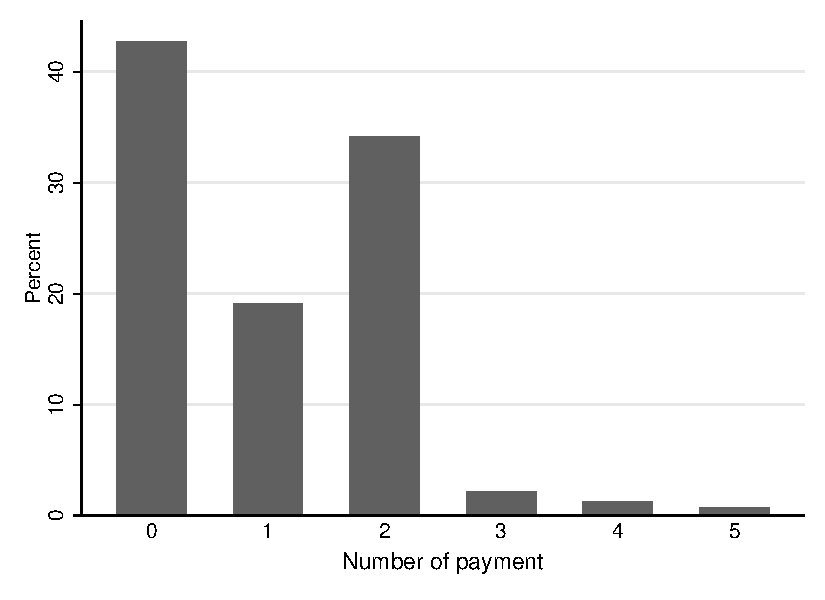
\includegraphics[width=\textwidth]{Figuras/hist_numpay_default.pdf}
    \end{subfigure}
    \end{center}
        \scriptsize 
        This figure describes behavior for the subsample of clients whose pawn was not recovered (in the control group).  Panel (a) shows days elapsed from the pawn to the first payment, while panel (b) displays the days elapsed to last payment. Some people pay after the day 105 when the grace period ends because the can ``restart'' the loan if they pay all interest owed. It amounts to starting a new loan with the same conditions and same pawn. Panel (c) shows the fraction of the loan that they paid (even when they ended up losing the pawn). Panel (d) displays the number of times they went to the branch to pay.      
      %\textit{Do file: }  \texttt{hist\_den\_default.do}
\end{figure}


\newpage
\subsection{Main treatment effects: Additional material}



\begin{figure}[H]
        \caption{Financial cost for different discount rates}
    \label{fc_discount_rates}
    \begin{center}
        \centering
        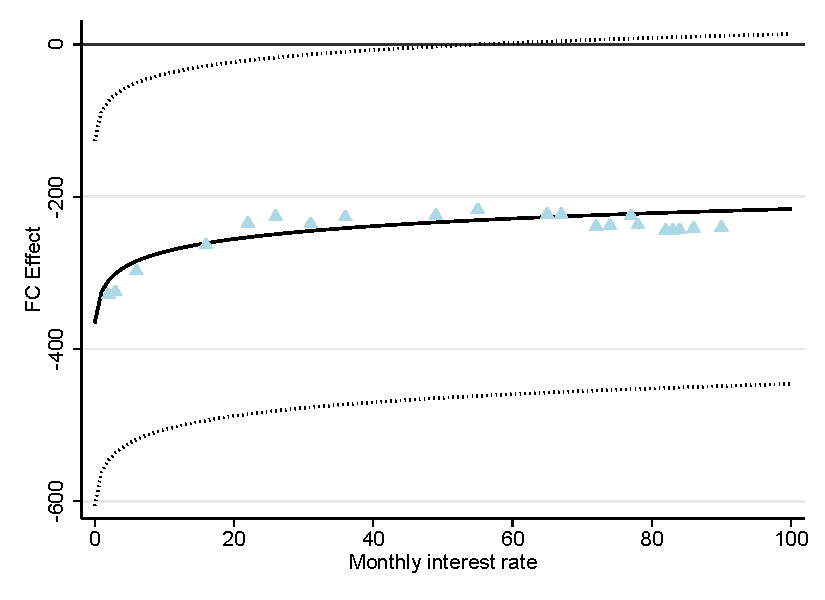
\includegraphics[width=0.55\textwidth]{Figuras/discount_effect.pdf}
    \end{center}
     \scriptsize This Figure estimates the treatment effect on financial cost with different discount rates.  
     %\textit{Do file: }  \texttt{discounted\_noeffect.do}
\end{figure}

\begin{landscape}

\begin{table}[H]
\caption{Multiple-loans robustness check}
\label{multiple_loans}
\begin{center}
\scriptsize{% Table generated by Excel2LaTeX from sheet 'multiple_loans'
\begin{tabular}{lccccccccccc}
\toprule
      & \multicolumn{3}{c}{Baseline approach} &       & \multicolumn{3}{c}{First treatment} &       & \multicolumn{3}{c}{ITT} \\
\cmidrule{2-4}\cmidrule{6-8}\cmidrule{10-12}      & FC    & APR   & Default &       & FC    & APR   & Default &       & FC    & APR   & Default \\
\midrule
      & (1)   & (2)   & (3)   &       & (4)   & (5)   & (6)   &       & (7)   & (8)   & (9) \\
\midrule
\midrule
Forced commitment & -408.0*** & -39.9*** & -0.12*** &       & -373.0** & -50.7*** & -0.16*** &       & -339.5*** & -40.4*** & -0.12*** \\
      & (134.9) & (6.40) & (0.022) &       & (148.7) & (7.24) & (0.026) &       & (121.4) & (5.91) & (0.022) \\
Choice commitment & -159.5 & 1.62  & -0.0022 &       & -103.2 & 0.079 & -0.011 &       & -55.1 & -4.62 & -0.030 \\
      & (128.9) & (6.42) & (0.019) &       & (146.6) & (7.76) & (0.024) &       & (124.9) & (6.00) & (0.019) \\
      &       &       &       &       &       &       &       &       &       &       &  \\
\midrule
Observations & 8510  & 8510  & 8510  &       & 6299  & 6299  & 6299  &       & 8806  & 8806  & 8806 \\
R-squared & 0.010 & 0.038 & 0.021 &       & 0.007 & 0.039 & 0.024 &       & 0.011 & 0.035 & 0.022 \\
Control Mean & 3270.6 & 249.1 & 0.56  &       & 3297.9 & 258.1 & 0.59  &       & 3211.0 & 252.9 & 0.58 \\
\midrule
\midrule
      &       &       &       &       &       &       &       &       &       &       &  \\
\midrule
      & \multicolumn{11}{c}{Consolidated outcomes} \\
\midrule
      & \multicolumn{3}{c}{Baseline approach} &       & \multicolumn{3}{c}{First treatment} &       & \multicolumn{3}{c}{ITT} \\
\cmidrule{2-4}\cmidrule{6-8}\cmidrule{10-12}      & FC    & APR   & Default &       & FC    & APR   & Default &       & FC    & APR   & Default \\
\midrule
      & (10)  & (11)  & (12)  &       & (13)  & (14)  & (15)  &       & (16)  & (17)  & (18) \\
\midrule
\midrule
Forced commitment & -1026.1*** & -38.7*** & -0.13*** &       & -896.9*** & -47.6*** & -0.16*** &       & -793.2*** & -42.0*** & -0.14*** \\
      & (219.8) & (5.44) & (0.019) &       & (222.2) & (6.12) & (0.020) &       & (194.8) & (5.20) & (0.017) \\
Choice commitment & -345.9 & -4.35 & -0.022 &       & -222.3 & -6.35 & -0.037* &       & -1.41 & -12.0** & -0.051*** \\
      & (234.4) & (5.18) & (0.017) &       & (237.1) & (5.94) & (0.020) &       & (241.7) & (4.77) & (0.016) \\
      &       &       &       &       &       &       &       &       &       &       &  \\
Observations & 5941  & 5941  & 5941  &       & 4438  & 4438  & 4438  &       & 6102  & 6102  & 6102 \\
R-squared & 0.013 & 0.032 & 0.020 &       & 0.012 & 0.035 & 0.024 &       & 0.014 & 0.030 & 0.022 \\
Control Mean & 4853.3 & 242.7 & 0.57  &       & 4755.9 & 248.5 & 0.59  &       & 4676.9 & 246.9 & 0.59 \\
\bottomrule
\bottomrule
\end{tabular}%
}
\end{center}
 \scriptsize

%\textit{Do file: } \texttt{multiple\_loans.do}
\end{table}

\end{landscape}


\begin{figure}[H]
        \caption{Survival graph}
    \label{survival_graph}
    \begin{center}
   \begin{subfigure}{0.49\textwidth}
   \caption{Ended contract}
        \centering
        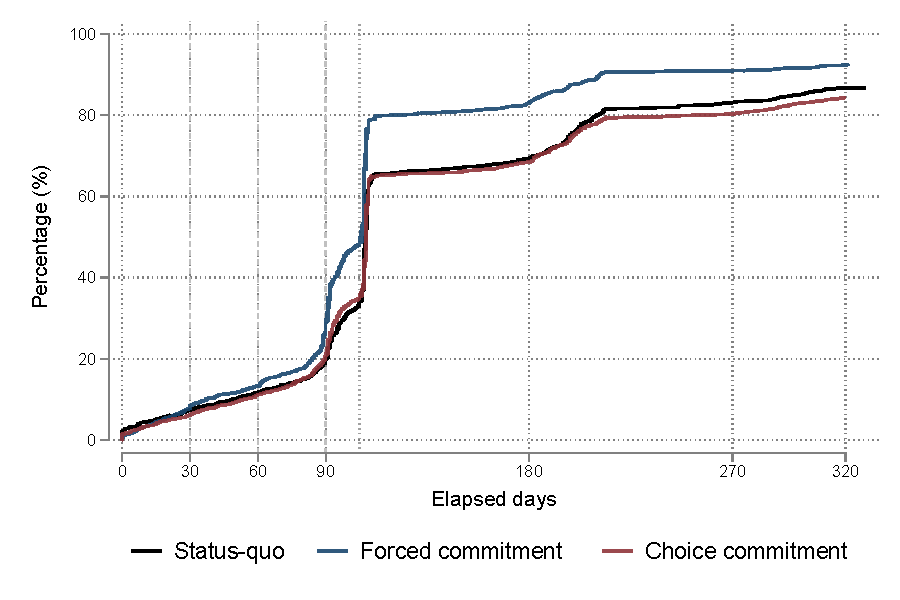
\includegraphics[width=\textwidth]{Figuras/survival_graph_ended.pdf}
    \end{subfigure} 
   \begin{subfigure}{0.49\textwidth}
   \caption{Recovery}
        \centering
        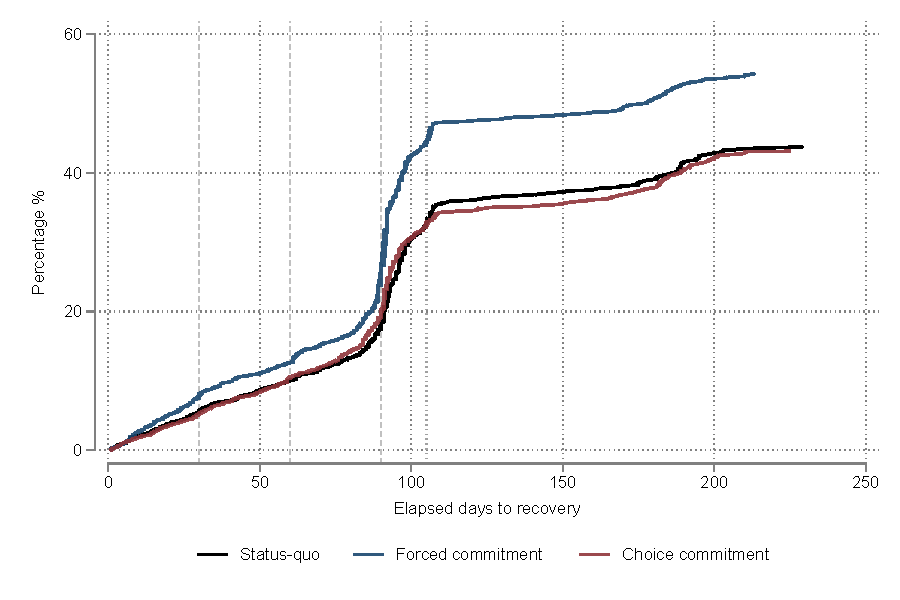
\includegraphics[width=\textwidth]{Figuras/survival_graph_unpledge.pdf}
    \end{subfigure}     
    \end{center}
     \scriptsize  This Figure shows the accumulated percentage of recovery in time by treatment arm. 
     %\textit{Do file: }  \texttt{survival\_graph.do}
\end{figure}

\begin{figure}[H]
        \caption{\% of payment over time}
    \label{porc_payment_over_time}
    \begin{center}
   \begin{subfigure}{0.49\textwidth}
        \caption{Unconditional}
        \centering
        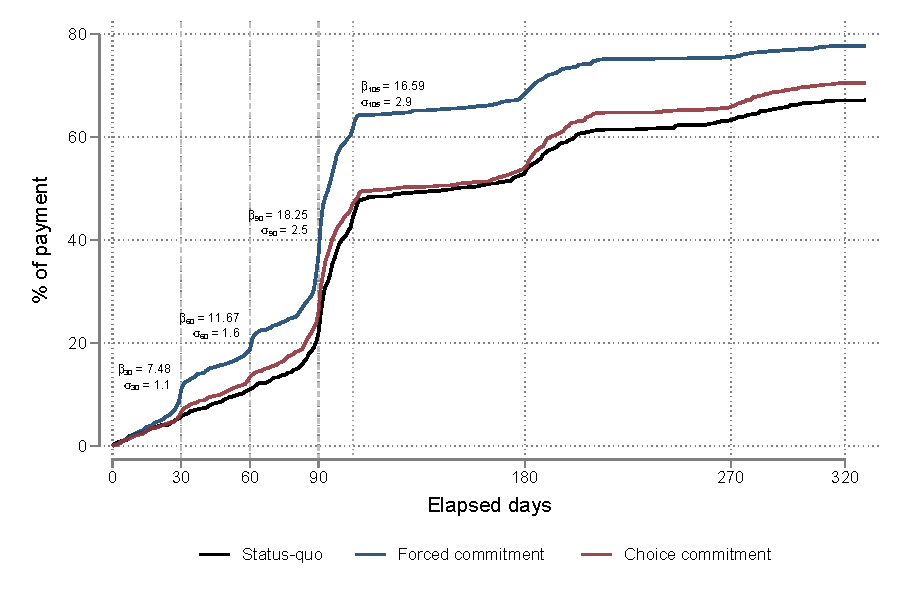
\includegraphics[width=\textwidth]{Figuras/cumulative_porc_pay_time.pdf}
    \end{subfigure} 
   \begin{subfigure}{0.49\textwidth}
        \caption{Conditional on default}
        \centering
        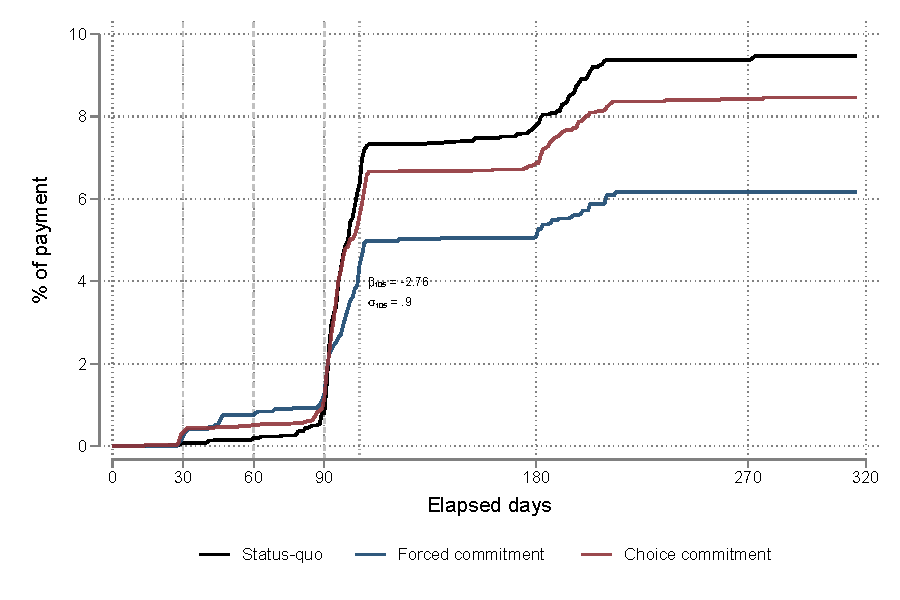
\includegraphics[width=\textwidth]{Figuras/cumulative_porc_pay_time_default.pdf}
    \end{subfigure}     
    \end{center}
     \scriptsize  This Figure shows the accumulated percentage of recovery in time by treatment arm. 
     %\textit{Do file: }  \texttt{cumulative\_porc\_pay\_time.do}
\end{figure}






\cleardoublepage


\vspace{.2in}
\begin{figure}[H]
        \caption{Empirical CDF of Financial Cost: fee-focing vs status-quo}
    \label{ecdf_fc}
    \begin{center}
        \centering
        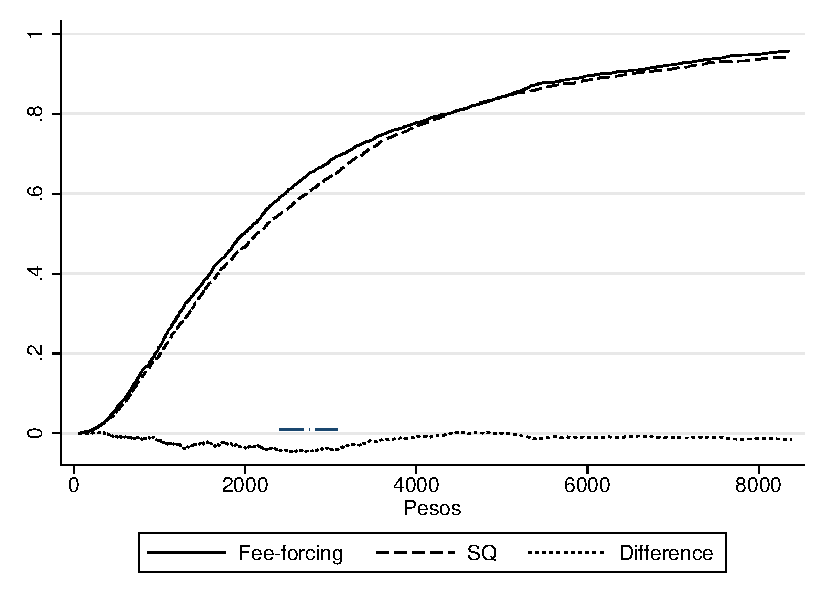
\includegraphics[width=0.65\textwidth]{Figuras/cdf_fc_pro_2.pdf}
    \end{center}
    \scriptsize This figure plots the empirical cumulative distribution of financial cost. It does this separately for the fee-forcing contract and for the status-quo contract. The doted line at the bottom is the difference of the status-quo CDF minus the fee-forcing CDF. It shows that the CDF of the status quo contract is always below that of the fee-forcing (and this difference is significant for the points indicated by the blue line), and therefore that the former first-order stochastically dominates the later for weakly decreasing utility functions; see Proposition \ref{eq_fosd}.
    % \texttt{ecdf\_fc.do}}
\end{figure}

\begin{figure}[H]
        \caption{Empirical CDF of APR: fee-focing vs status-quo}
    \label{ecdf_fc}
    \begin{center}
        \centering
        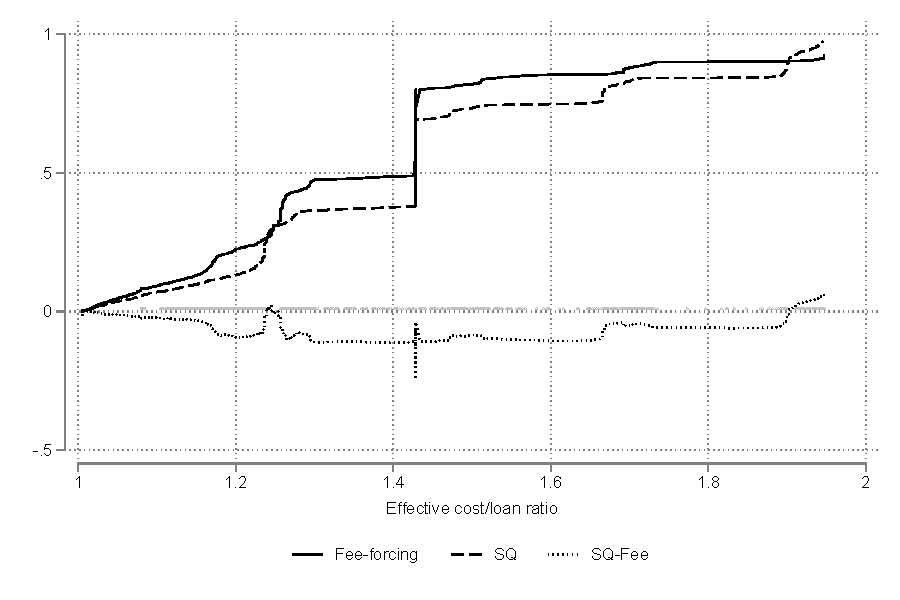
\includegraphics[width=0.65\textwidth]{Figuras/cdf_eff_pro_2.pdf}
    \end{center}
    \scriptsize This figure plots the empirical cumulative distribution of financial cost. It does this separately for the fee-forcing contract and for the status-quo contract. The doted line at the bottom is the difference of the status-quo CDF minus the fee-forcing CDF. It shows that the CDF of the status quo contract is always below that of the fee-forcing (and this difference is significant for the points indicated by the blue line), and therefore that the former first-order stochastically dominates the later for weakly decreasing utility functions; see Proposition \ref{eq_fosd}.
    % \texttt{ecdf\_eff.do}}
\end{figure}


\vspace{.2in}
\begin{table}[H]
\caption{Clients who should prefer fee-forcing financial cost distribution}
\label{stochastic_dominance}
\begin{center}
\scriptsize{% Table generated by Excel2LaTeX from sheet 'dominance'
\begin{tabular}{lccc}
\toprule
Sub-population & Dominance & Log-normality (AD/KS) & Obs \\
\midrule
\midrule
Fee-forcing & \cellcolor[rgb]{ .557,  .663,  .859} $\succeq_{1}^*$ & */*  |  */* & 5034 \\
Low-loan & $\succeq_{1}^*$ &    /     |     /    & 2508 \\
High-loan & $\succeq_{1}^*$ &    /     |     /    & 2526 \\
Low-subj. prob. & \cellcolor[rgb]{ .557,  .663,  .859} $\succeq_{1}^*$ & */*  |  */* & 1083 \\
High-subj. Prob. & \cellcolor[rgb]{ .557,  .663,  .859} $\succeq_{1}^*$ & */*  |  */* & 2590 \\
Low-age & $\preceq_{1}$ & */*  |  */* & 1358 \\
High-age & \cellcolor[rgb]{ .851,  .882,  .949} $\succeq_{1}$ & */*  |     /* & 1362 \\
Low-income index & \cellcolor[rgb]{ .851,  .882,  .949} $\succeq_{1}$ & */*  |  */* & 1047 \\
High-income index & \cellcolor[rgb]{ .851,  .882,  .949} $\succeq_{1}$ & */*  |  */* & 948 \\
Male  & -     & */*  |     /* & 755 \\
Female & \cellcolor[rgb]{ .851,  .882,  .949} $\succeq_{1}$ & */*  |  */* & 2158 \\
First time & $\preceq_{1}$ & */*  |  */* & 293 \\
Pawn before & \cellcolor[rgb]{ .851,  .882,  .949} $\succeq_{1}$ & */*  |  */* & 2475 \\
Family doesn't ask & $\preceq_{1}$ & */*  |  */* & 1826 \\
Family asks & \cellcolor[rgb]{ .557,  .663,  .859} $\succeq_{1}^*$ & */*  |  */* & 987 \\
Not common ask & \cellcolor[rgb]{ .851,  .882,  .949} $\succeq_{1}$ & */*  |  */* & 1436 \\
Common asks & -     & */*  |  */* & 625 \\
No savings & $\preceq_{1}$ & */*  |  */* & 1353 \\
Has savings & \cellcolor[rgb]{ .557,  .663,  .859} $\succeq_{1}^*$ & */*  |  */* & 717 \\
Not rosca & \cellcolor[rgb]{ .557,  .663,  .859} $\succeq_{1}^*$ & */*  |  */* & 1270 \\
Rosca & $\preceq_{1}$ & */*  |  */* & 795 \\
Low-education & \cellcolor[rgb]{ .851,  .882,  .949} $\succeq_{1}$ & */*  |     /* & 906 \\
High-education & \cellcolor[rgb]{ .851,  .882,  .949} $\succeq_{1}$ & */*  |  */* & 1797 \\
Not stressed & -     & */*  |  */* & 1998 \\
Stressed & -     & */*  |  */* & 839 \\
Not overconfident & $\preceq_{1}$ & */*  |  */* & 47 \\
Overconfident & \cellcolor[rgb]{ .851,  .882,  .949} $\succeq_{1}$ & */*  |     /* & 1626 \\
Not PB & \cellcolor[rgb]{ .851,  .882,  .949} $\succeq_{1}$ & */*  |  */* & 1438 \\
PB    & \cellcolor[rgb]{ .557,  .663,  .859} $\succeq_{1}^*$ & */*  |     /* & 226 \\
Not FB & \cellcolor[rgb]{ .851,  .882,  .949} $\succeq_{1}$ & */*  |  */* & 1521 \\
FB    & \cellcolor[rgb]{ .851,  .882,  .949} $\succeq_{1}$ & */*  |  */* & 143 \\
Doesn't make budget & \cellcolor[rgb]{ .851,  .882,  .949} $\succeq_{1}$ & */*  |  */* & 1054 \\
Makes budget & \cellcolor[rgb]{ .851,  .882,  .949} $\succeq_{1}$ & */*  |  */* & 1689 \\
Not tempted & \cellcolor[rgb]{ .851,  .882,  .949} $\succeq_{1}$ & */*  |     /* & 875 \\
Tempted & \cellcolor[rgb]{ .851,  .882,  .949} $\succeq_{1}$ & */*  |  */* & 1872 \\
High-transp. cost & \cellcolor[rgb]{ .851,  .882,  .949} $\succeq_{1}$ & */*  |  */* & 1352 \\
Low-transp. cost & \cellcolor[rgb]{ .851,  .882,  .949} $\succeq_{1}$ & */*  |  */* & 1343 \\
High-transp. time & \cellcolor[rgb]{ .851,  .882,  .949} $\succeq_{1}$ & */*  |  */* & 1260 \\
Low-transp. time & \cellcolor[rgb]{ .557,  .663,  .859} $\succeq_{1}^*$ & */*  |  */* & 1442 \\
\bottomrule
\bottomrule
\end{tabular}%
}
\end{center}
 \footnotesize
This table does two things. First, it tests whether the observed empirical distribution of financial cost is well approximated by a log normal. It does this using two tests, the Anderson-Darling and the Kolmogorov-Smirnoff tests. Second, it fits a log normal distribution by maximum likelihood to observed empirical distribution of financial cost, separately for the fee-forcing arm and the status-quo arm. Using the fitted log normal, it tests whether the fee-forcing financial cost distribution would be preferred by any expected utility agent using Proposition \ref{lognormal_fosd} below. The different rows of the table do this for different sub-populations.  The first row of the table does it for every client in the fee forcing and status quo arms. The ``*'' show that we cannot reject at the 5\% level that both distribution are log normal for any of the two tests. The column entitled ``Dominance'' shows whether any client that dislikes higher cost would prefer the fee-forcing cost distribution over the status quo one, with $\succeq_{1}$ meaning he should (with $\succeq_{1}^*$ indicating the difference is statistically significant). It turns out to be the case that for the overwhelming majority of sub-populations, the conditions of preferring the fee-forcing distribution hold.
%\textit{Do file: } \texttt{stoch\_dominance.do}
\end{table}


\vspace{.2in}
\begin{prop}
\label{lognormal_fosd}
\footnotesize{
Let $F$ and $G$ be the cumulative distributions of two alternative log-normal prospects. The following are equivalent:

\begin{enumerate}[(a)]
    \item For every weakly decreasing utility function $u$: $E_{F}(u(FC))\leq E_G(u(FC))$
    \item $E_F \log(FC)\geq E_G\log(FC)$ and $Var_F \log(FC)= Var_G\log(FC)$
\end{enumerate}
}
\end{prop}

\begin{proof}
\footnotesize{
See Theorem 4 in \cite{lognormal_dominance}.
}
\end{proof}

\newpage

\vspace{.1in}
\begin{prop}
\label{eq_fosd}
\footnotesize{
This is a standard result. 
\\
\vspace{.1in}
The following are equivalent:
\begin{enumerate}[(a)]
    \item For every weakly decreasing utility function $u$: $E_{sq}(u(FC))\leq E_{fee}(u(FC))$
    \item $F_{sq}(FC)\leq F_{fee}(FC)$ 
\end{enumerate}
}
\end{prop}
\begin{proof} \;
\footnotesize{

[$(a)\Longrightarrow (b)$] Suppose  $(b)$ does not hold. So there exists $FC^*$ such that $F_{sq}(FC^*)>F_{fee}(FC^*)$, Define $u:=\mathds{1}_{FC\leq FC^*}$. Then
\[E_{sq}(u(FC)) = \int u(FC)dF_{sq} = F_{sq}(FC^*)>F_{fee}(FC^*)= \int u(FC)dF_{fee} =E_{fee}(u(FC))\]
which contradicts $(a)$.\\

[$(a)\Longleftarrow (b)$] On the other hand for $u$ weakly decreasing,

\[\int u(y(FC))dF_{sq}(y(FC)) = \int u(y(FC))dF_{fee}(FC) \leq \int u(FC)dF_{fee}(FC)\]
with $y(FC) = F_{sq}^{-1}F_{fee}(FC)$.
}
\end{proof}
\footnotesize{
Note the proof was done in the case of absolutely continuous and strictly increasing distribution functions $F_{sq}$ and $F_{fee}$.
}



\newpage


\subsection{Testing for heterogeneity}
Our approach relies on the following simple observation: if $\Delta_i$ is constant across $i$ then we must have 
\[
\text{ATE}(X_i) \equiv \mathbbm{E}[\Delta_i |X_i] = \mathbbm{E}[\Delta_i] \equiv \text{ATE}
\]
for any covariates $X_i$ that vary across $i$. If, on the other hand, $\text{ATE}(X_i)$ can be predicted using some scalar function $\tau(\cdot)$ of $X_i$, then the average treatment effect function is not constant so there must be treatment effect heterogeneity. 

We operationalize this idea using a two-step approach proposed by \cite{chernozhukov2018generic}.  We begin by randomly dividing the participants in the forced arms of the experiment ($Z_i \neq 2$) into two groups: a ``training set'' and a \todo{80/20 split?}{``test set.''} In the first step, we apply random forests to the training set to estimate two proxy predictors: $\psi(\cdot|\text{Training})$ approximates the untreated potential outcome function, $\mathbbm{E}[Y_{i0}|X_i] = \mathbbm{E}[Y_i|Z_i=0,X_i]$, while  $\tau(\cdot|\text{Training})$, approximates the average treatment effect function
\[
\text{ATE}(X_i) = \mathbbm{E}[Y_i|Z_i=1,X_i] - \mathbbm{E}[Y_i|Z_i=0, X_i].
\]
The proxy predictors need not be unbiased or even consistent estimators of the functions they aim to approximate: the goal of this exercise is merely to find a scalar function of $X_i$ that \emph{accurately predicts} $\text{ATE}(X_i)$.

In the second step we fit a linear regression model to data from the training set using regressors constructed from the proxy functions $\psi(\cdot|\text{Training})$ and $\tau(\cdot|\text{Training})$ constructed in the first step. In particular, we estimate 
\begin{equation}
Y_i = \alpha_0 + \alpha_1 \psi_i + \beta_1 (Z_i - \mathbbm{E}[Z_i]) + \beta_2 (Z_i - \mathbbm{E}[Z_i])(\tau_i - \mathbbm{E}[\tau_i]) + \epsilon_i
\label{eq:chernreg}
\end{equation}
where $\psi_i \equiv \psi(X_i|\text{Training})$ and $\tau_i \equiv \tau(X_i|\text{Training})$.\footnote{This is a slightly simpler regression than the one proposed in equation (3.1) of \cite{chernozhukov2018generic}, which involves propensity score weights. Because the random assignment of $Z$ in our experiment does \emph{not} condition on $X$, the propensity score weights in our case are constant over $X$ and hence drop out.} As shown by \cite{chernozhukov2018generic}, the coefficients $\beta_1$ and $\beta_2$ from \eqref{eq:chernreg} identify the \emph{best linear predictor} of the conditional ATE based on $\tau(\cdot|\text{Training})$, namely
\[
\beta_1 = \mathbbm{E}[\text{ATE}(X_i)] = \text{ATE}, \quad
\beta_2 = \frac{\text{Cov}[\text{ATE}(X_i), \tau_i]}{\text{Var}(\tau_i)}.
\]
If treatment effects are homogeneous we must have $\beta_2 = 0$. Rejecting this hypothesis establishes that $\tau_i$ predicts $\text{ATE}(X_i)$ and hence that $\Delta_i$ varies. Since $\tau_i$ and $\psi_i$ do not depend on the test set, inference for the regression in \eqref{eq:chernreg} is straightforward conditional on the Training/Test split.  

\todo[inline]{Discuss the results here.}

\todo[inline]{Issac: re-run this exercise with removing the propensity score weights $p(Z)$. Presumably it shouldn't change anything, but it's simpler to explain what we do and probably less noisy

\begin{table}[H]
\begin{center}
\scriptsize{% Table generated by Excel2LaTeX from sheet 'test_calibration_2'
\begin{tabular}{rccccc}
\toprule
      & \multicolumn{5}{c}{Test Calibration} \\
\midrule
      & \multicolumn{2}{c}{With PS} &       & \multicolumn{2}{c}{Without PS} \\
\cmidrule{2-3}\cmidrule{5-6}      & \multicolumn{2}{c}{APR} &       & \multicolumn{2}{c}{APR} \\
\cmidrule{2-3}\cmidrule{5-6}      & BVC   & BVC + survey variables &       & BVC   & BVC + survey variables \\
\midrule
      & (1)   & (2)   &       & (3)   & (4) \\
\midrule
\midrule
\multicolumn{1}{l}{Mean Forest Prediction} & 0.9797 & 0.9983 &       & 0.8302 & 0.8816 \\
      & (0.1335) & (0.1165) &       & (0.1198) & (0.1034) \\
\multicolumn{1}{l}{Differential Forest Prediction} & 0.9486 & 1.3224 &       & 0.8107 & 1.2027 \\
      & (0.1270) & (0.2073) &       & (0.1163) & (0.1861) \\
\bottomrule
\bottomrule
\end{tabular}%
}
\end{center}
\end{table}

}

\todo[inline]{Some Questions for Issac: (1) How are we carrying out the sample splitting? If we cluster standard errors at the branch-day level, we should take this into account when we split. (2) How are you carrying out inference for $\beta_2$? Chernozhukov et al discuss two approaches: ``conditional'' and ``variational.'' The former is simpler as it conditions on the training/test split. The latter is a bit more involved, since one accounts for uncertainty arising from different splits. (3) What are the details of the random forest procedure employed here? (Tuning parameters choice, etc.) We should put them into the appendix.}





\newpage

\subsection{Bounding ToT \& TuT} \label{bound_tot_tut_appendix}

\vspace{.2in}
\normalsize
\linespread{1.25}
%Really force it to normal size and linespread
\normalsize
\linespread{1.25}

Even without the exclusion restriction, it’s possible to bound $\mathbb{E}[Y_1-Y_0\;|\;T=0]$ and $\mathbb{E}[Y_1-Y_0\;|\;T=1]$ using observed outcomes in the forced arm and observed take-up in the choice arm. It should also be possible to create bounds conditional on covariates. The basic approach is similar to that of \cite{huber_mellace}. \\


From the $Z=0$ arm we identify the distribution $F_0$ of $Y_0$, the potential outcome when forced into the no-commitment contract. Now, from the choice arm we know that around 90\% of people are $T=0$ types. Because choice was randomly assigned, the 90\% figure holds for all arms in the experiment. This tells us that $F_0$ is a 90\%-10\% mixture of $Y_0\;|\;T=0$ and $Y_0\;|\;T=1$. Cut out the bottom 10\% of $F_0$ and calculate the mean of this new distribution. Then cut out the top 10\% of $F_0$ and compute the mean of this new distribution. The result is an upper and lower bound for $\mathbb{E}[Y_0\;|\;T=0]$ that does not rely on the exclusion restriction. We can apply similar reasoning to bound $\mathbb{E}[Y_1\;|\;T=0]$ Combining the previous bounds gives a bound for the TuT that does not rely on the exclusion restriction, and analogous we can bound the ToT. \\



The \cite{huber_mellace} bounds for the ToT \& TuT APR are respectively:
\[\text{ToT} : [-481.8, 483.7]\quad\quad\quad\text{TuT} : [-17.9, 90.6]\]

Note that since both TuT and ToT estimates from the LATE approach lies inside these bounds, we do not falsify the exclusion restriction. 


\newpage





\subsection{LATE: ToT \& TuT}
\vspace{.2in}
\normalsize
\linespread{1.25}
%Really force it to normal size and linespread
\normalsize
\linespread{1.25}

 Recall that $Z_i$ is the observed, randomly assigned experimental allocation, where $Z_i=0$ denotes the control arm, $Z_i=1$ denotes the forced-fee arm, and $Z_i=2$ is the choice arm.  Let $C_i$ be the unobserved choice type. $C_i=0$ when individual $i$ does not choose commitment  given the choice and $C_i=1$ when chooses commitment given the choice. Finally, $D_i = Z_i\times \mathds{1}(Z_i\neq 2) + C_i\times \mathds{1}(Z_i=2)$ is the observed treatment indicator, and $Y(d,z)$ is the potential outcome function for $d=0,1$, and $z=0,1,2$. 

 To identify assortative selection we first need to estimate the following quantities: $\mathbb{E}(Y_1-Y_0\;|\;C=1)$ the Treatment on the Treated (ToT), and $\mathbb{E}(Y_1-Y_0\;|\;C=0)$ the Treatment on the Untreated (TuT). 

 To point identify the above quantities, we make the following assumptions.

 \begin{assumption}[Exclusion Restriction]
$Z$ only affects $Y$ through its effect on $D$ : $C(d,z) = C(d)$
 \end{assumption}

  \begin{assumption}[Independence Assumption]
$Z \perp (Y_0, Y_1, C)$
 \end{assumption}

The following intermediate Lemmas will help us derive that both ToT and TuT are point identified.

\begin{lem}
$\Pr(C=1) = \E[D\;|\;Z=2]$
\end{lem}
\begin{proof}
Since $C\perp Z$, 
$$\E[D\;|\;Z=2] = \E[Z\times \mathds{1}(Z\neq 2)+ C\times\mathds{1}(Z=2)\;|Z=2] = \E[C\;|\;Z=2] = \E[C] = \Pr(C=1)$$
\end{proof}


\begin{lem}
$\E[Y_0] = \E[Y\;|\;Z=0]$
\end{lem}
\begin{proof}
Since $Z\perp Y_0$, 
\begin{align*}
\E[Y\;|\;Z=0] =& \E[\mathds{1}(Z=0)Y_0+\mathds{1}(Z=1)Y_1+\mathds{1}(Z=2)\{(1-C)Y_0+CY_1\})\;|\;Z=0]\\   
=&\E[Y_0\;|\;Z=0] = \E[Y_0]
\end{align*}
\end{proof}


\begin{lem}
$\E[Y_1] = \E[Y\;|\;Z=1]$
\end{lem}
\begin{proof}
Since $Z\perp Y_1$, 
\begin{align*}
\E[Y\;|\;Z=1] =\E[Y_1\;|\;Z=1] = \E[Y_1]
\end{align*}
\end{proof}


\begin{lem}
$\E[Y_0\;|\;C=0] = \E[Y\;|\; D=0,Z=2]$
\end{lem}
\begin{proof}
If $Z=2$, then $D=0$ if and only if $C=0$. Hence,
\[\E[Y\;|\;D=0, Z=2] = \E[Y_0\;|\;D=0, Z=2] = E[Y_0\;|\;C=0, Z=2]=\E[Y_0\;|\;C=0]\]
since $Y_0\perp C\;|\;Z$
\end{proof}

\begin{lem}
$\E[Y_1\;|\;C=1] = \E[Y\;|\; D=1,Z=2]$
\end{lem}
\begin{proof}
If $Z=2$, then $D=1$ if and only if $C=1$. Hence,
\[\E[Y\;|\;D=1, Z=2] = \E[Y_1\;|\;D=1, Z=2] = E[Y_1\;|\;C=1, Z=2]=\E[Y_1\;|\;C=1]\]
since $Y_1\perp C\;|\;Z$
\end{proof}

\begin{theorem} $\E[Y_1-Y_0\;|\; C=1]$ is point identified
\end{theorem}

\begin{proof}
Since $\E[Y_1\;|\; C=1] = \E[Y\;|\; D=1, Z=2]$ by Lemma 5, it suffices to show that $\E[Y_1\;|\;C=0]$ is point identified. By iterated expectations:
\[E[Y_0] = \E_C\E[Y_0\;|\;C] = (1-p)\E[Y_0\;|\;C=0]+p\E[Y_0\;|\;C=1]\]
where $p:=\E[C]=\Pr(C=1)$, and re-arranging,
\[\E[Y_0\;|\;C=1] = \frac{1}{p}\left(E[Y_0] -(1-p)\E[Y_0\;|\;C=0]\right)\]
Finally, substituting the result of Lemmas 1, 2, and 4, we obtain
\[\E[Y_0\;|\;C=1] =\frac{1}{\E[D\;|\;Z=2]}\left\{\E[Y\;|\;Z=0]-(1-\E[D\;|\;Z=2])\E[Y\;|\;D=0, Z=2]\right\}\]
and the RHS is a function of observed data only.
\end{proof}

\begin{theorem} $\E[Y_1-Y_0\;|\; C=0]$ is point identified
\end{theorem}

\begin{proof}
Since $\E[Y_0\;|\; C=0] = \E[Y\;|\; D=0, Z=2]$ by Lemma 4, it suffices to show that $\E[Y_0\;|\;C=1]$ is point identified. By iterated expectations:
\[E[Y_1] = \E_C\E[Y_1\;|\;C] = (1-p)\E[Y_1\;|\;C=0]+p\E[Y_1\;|\;C=1]\]
where $p:=\E[C]=\Pr(C=1)$, and re-arranging,
\[\E[Y_1\;|\;C=0] = \frac{1}{1-p}\left(E[Y_1] -p\E[Y_1\;|\;C=1]\right)\]
Finally, substituting the result of Lemmas 1, 3, and 5, we obtain
\[\E[Y_1\;|\;C=0] =\frac{1}{1-\E[D\;|\;Z=2]}\left\{\E[Y\;|\;Z=1]-\E[D\;|\;Z=2]\E[Y\;|\;D=1, Z=2]\right\}\]
and the RHS is a function of observed data only.
\end{proof}


\begin{figure}[H]
    \caption{Bootstrap inference for the difference between ToT-TuT}
    \label{bootstrap_tot_tut}
    \begin{center}
    \begin{subfigure}{0.31\textwidth}
        \caption{Simple}
        \centering
        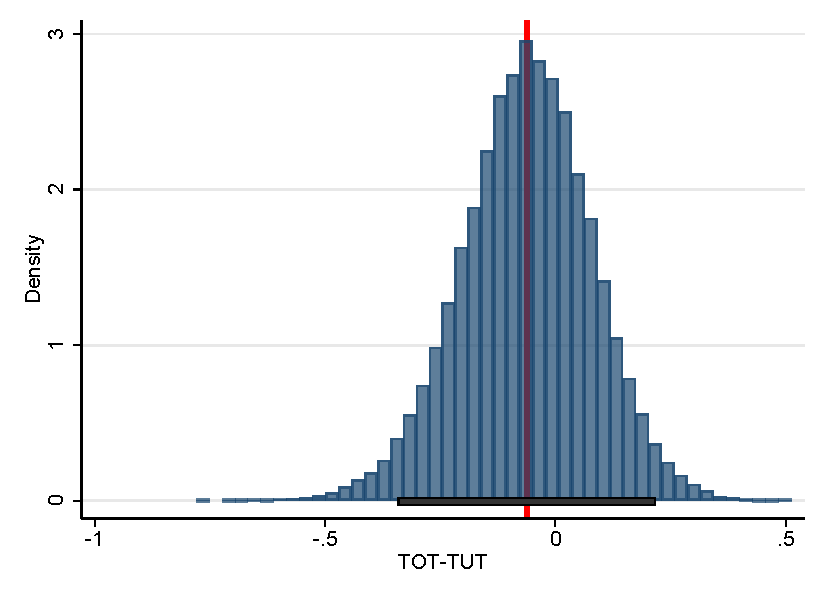
\includegraphics[width=\textwidth]{Figuras/tot_tut_btsp1.pdf}
    \end{subfigure}
    \begin{subfigure}{0.31\textwidth}
        \caption{Admin controls}
        \centering
        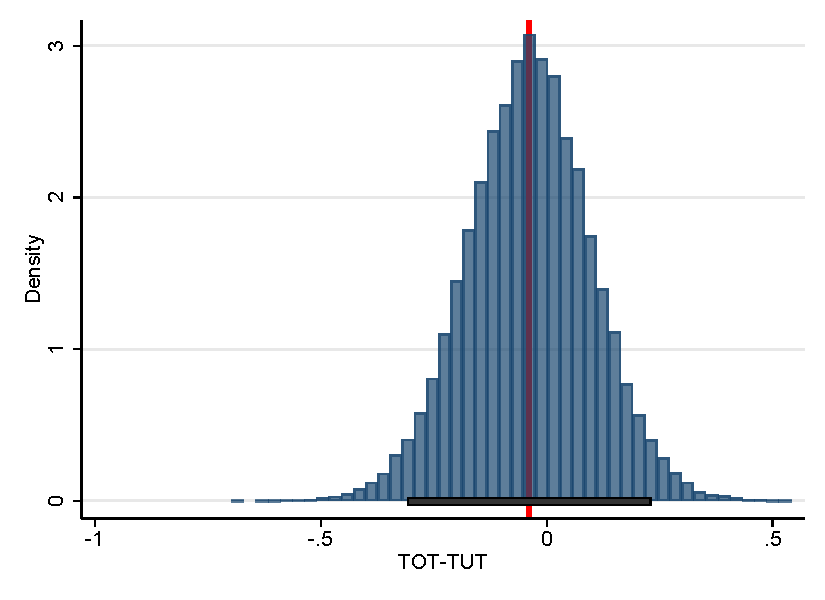
\includegraphics[width=\textwidth]{Figuras/tot_tut_btsp2.pdf}
    \end{subfigure}
    \begin{subfigure}{0.31\textwidth}
        \caption{Admin + Survey controls}
        \centering
        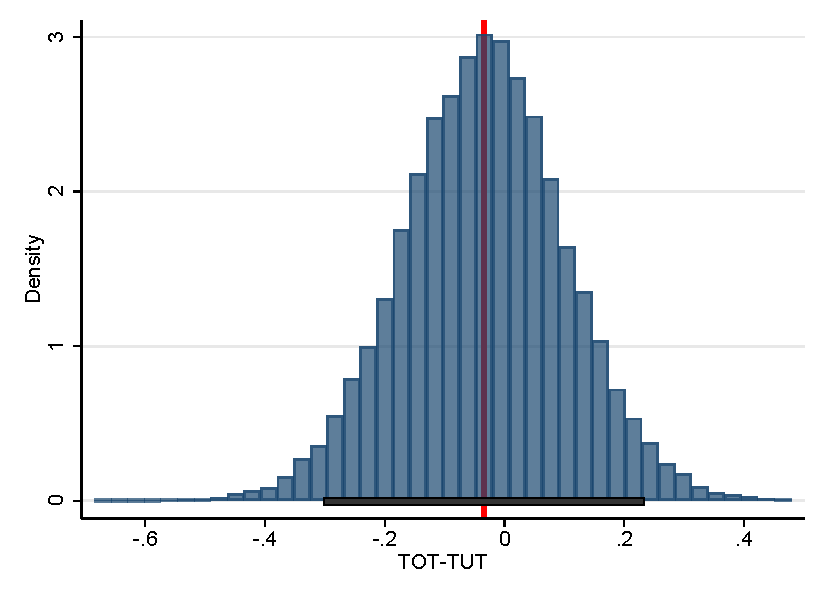
\includegraphics[width=\textwidth]{Figuras/tot_tut_btsp3.pdf}
    \end{subfigure}
  
    \end{center}
     \scriptsize  Given that all of the arms are effectively randomly sampled form the same pool, we can also estimate the ToT and TuT with the pooled regression: $Y_i = \beta_0\mathds{1}(Z_i=0)+\beta_1\mathds{1}(Z_i=1)+\beta_2\mathds{1}(Z_i=2)+ \epsilon_i$, and then this test statistic just becomes the F-test on $\frac{\widehat{\beta_2}-\widehat{\beta_0}}{p}$ for the ToT, $\frac{\widehat{\beta_1}-\widehat{\beta_2}}{1-p}$ for the TuT, and an F-test on the difference between these two quantities to test whether the gains are different between compliers and non-compliers. Recognizing the stochastic nature of the compliance rate, we also bootstrap this quantity before running the previous regression. The red line shows the point estimate for the difference between ToT-TuT, and the gray bar in the x-axis shows a 95\% confidence interval for this difference. Panel (a) shows the difference between the ToT and TuT without any controls, while panel (b) and (c) adds admin controls and admin + survey controls respectively.
          %\footnotesize{ \textit{Do file: }  \texttt{tot\_tut.do}}
\end{figure}


\begin{figure}[H]
     \caption{ToT-TuT CDF}
     \label{tot_tut_ecdf}
    \begin{center}
    \begin{subfigure}{0.6\textwidth}
        \centering
        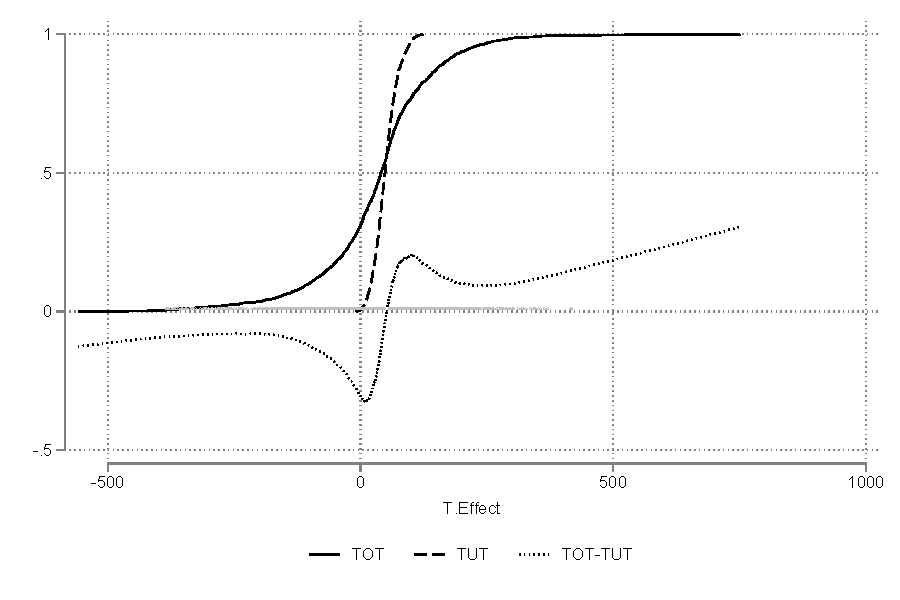
\includegraphics[width=\textwidth]{Figuras/cdf_tot_tut.pdf}
    \end{subfigure}
    \end{center}
    \scriptsize
       Equipped with estimates for the ToT and TuT for each individual $i$ from an Instrumental Random Forest we compute the ECDF for this quantities. The solid line is the ECDF for the ToT, the dashed line is the ECDF for the TuT, and the dotted line plots the difference between the ToT and the TuT - the blue dashed line in the x-axis shows the points where this difference is significant. The bold black interval at the bottom of the graph is the mean for the ToT distribution (0.07), while the gray interval shows the mean for the TuT distribution (0.10).
       
          %\footnotesize{ \textit{Do file: }  \texttt{tot\_tut\_insforest.do}}
\end{figure}

\begin{figure}[H]
     \caption{Exclusion restriction}
     \label{exclusion_restriction}
    \begin{center}
    \begin{subfigure}{0.6\textwidth}
        \centering
        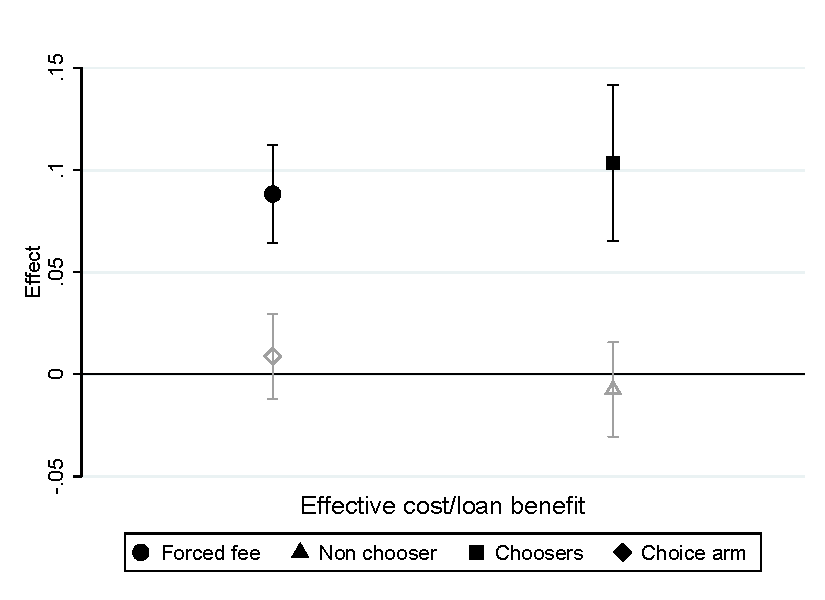
\includegraphics[width=\textwidth]{Figuras/exclusion_restriction.pdf}
    \end{subfigure}
    \end{center}
    \scriptsize This figure serves as a test for the exclusion restriction in the point identification for the ToT and the TuT. It shows the effect on the effective cost/loan ratio for the forced-fee arm and the choice arm, together with the decomposition of the choosers and non-choosers. Note that a) being forced into the treatment (Forced fee) has the same effect as choosing it (Choosers), and b) not choosing the treatment (Non chooser) has no effect with respect to the control.
    
          %\footnotesize{ \textit{Do file: }  \texttt{exclusion\_restriction.do}}
\end{figure}

%---------------------------------------------------------------------------------------------------------------------------------------------------------------------------------------------------------------------------------

\newpage 
\newpage
\subsection{Causal Random Forest and HTE}

\vspace{.3in}
\begin{figure}[H]
        \caption{Honest causal tree for the Forced-commitment contract heterogeneous treatment effects}
    \label{casual_tree}
    \begin{center}
        \centering
        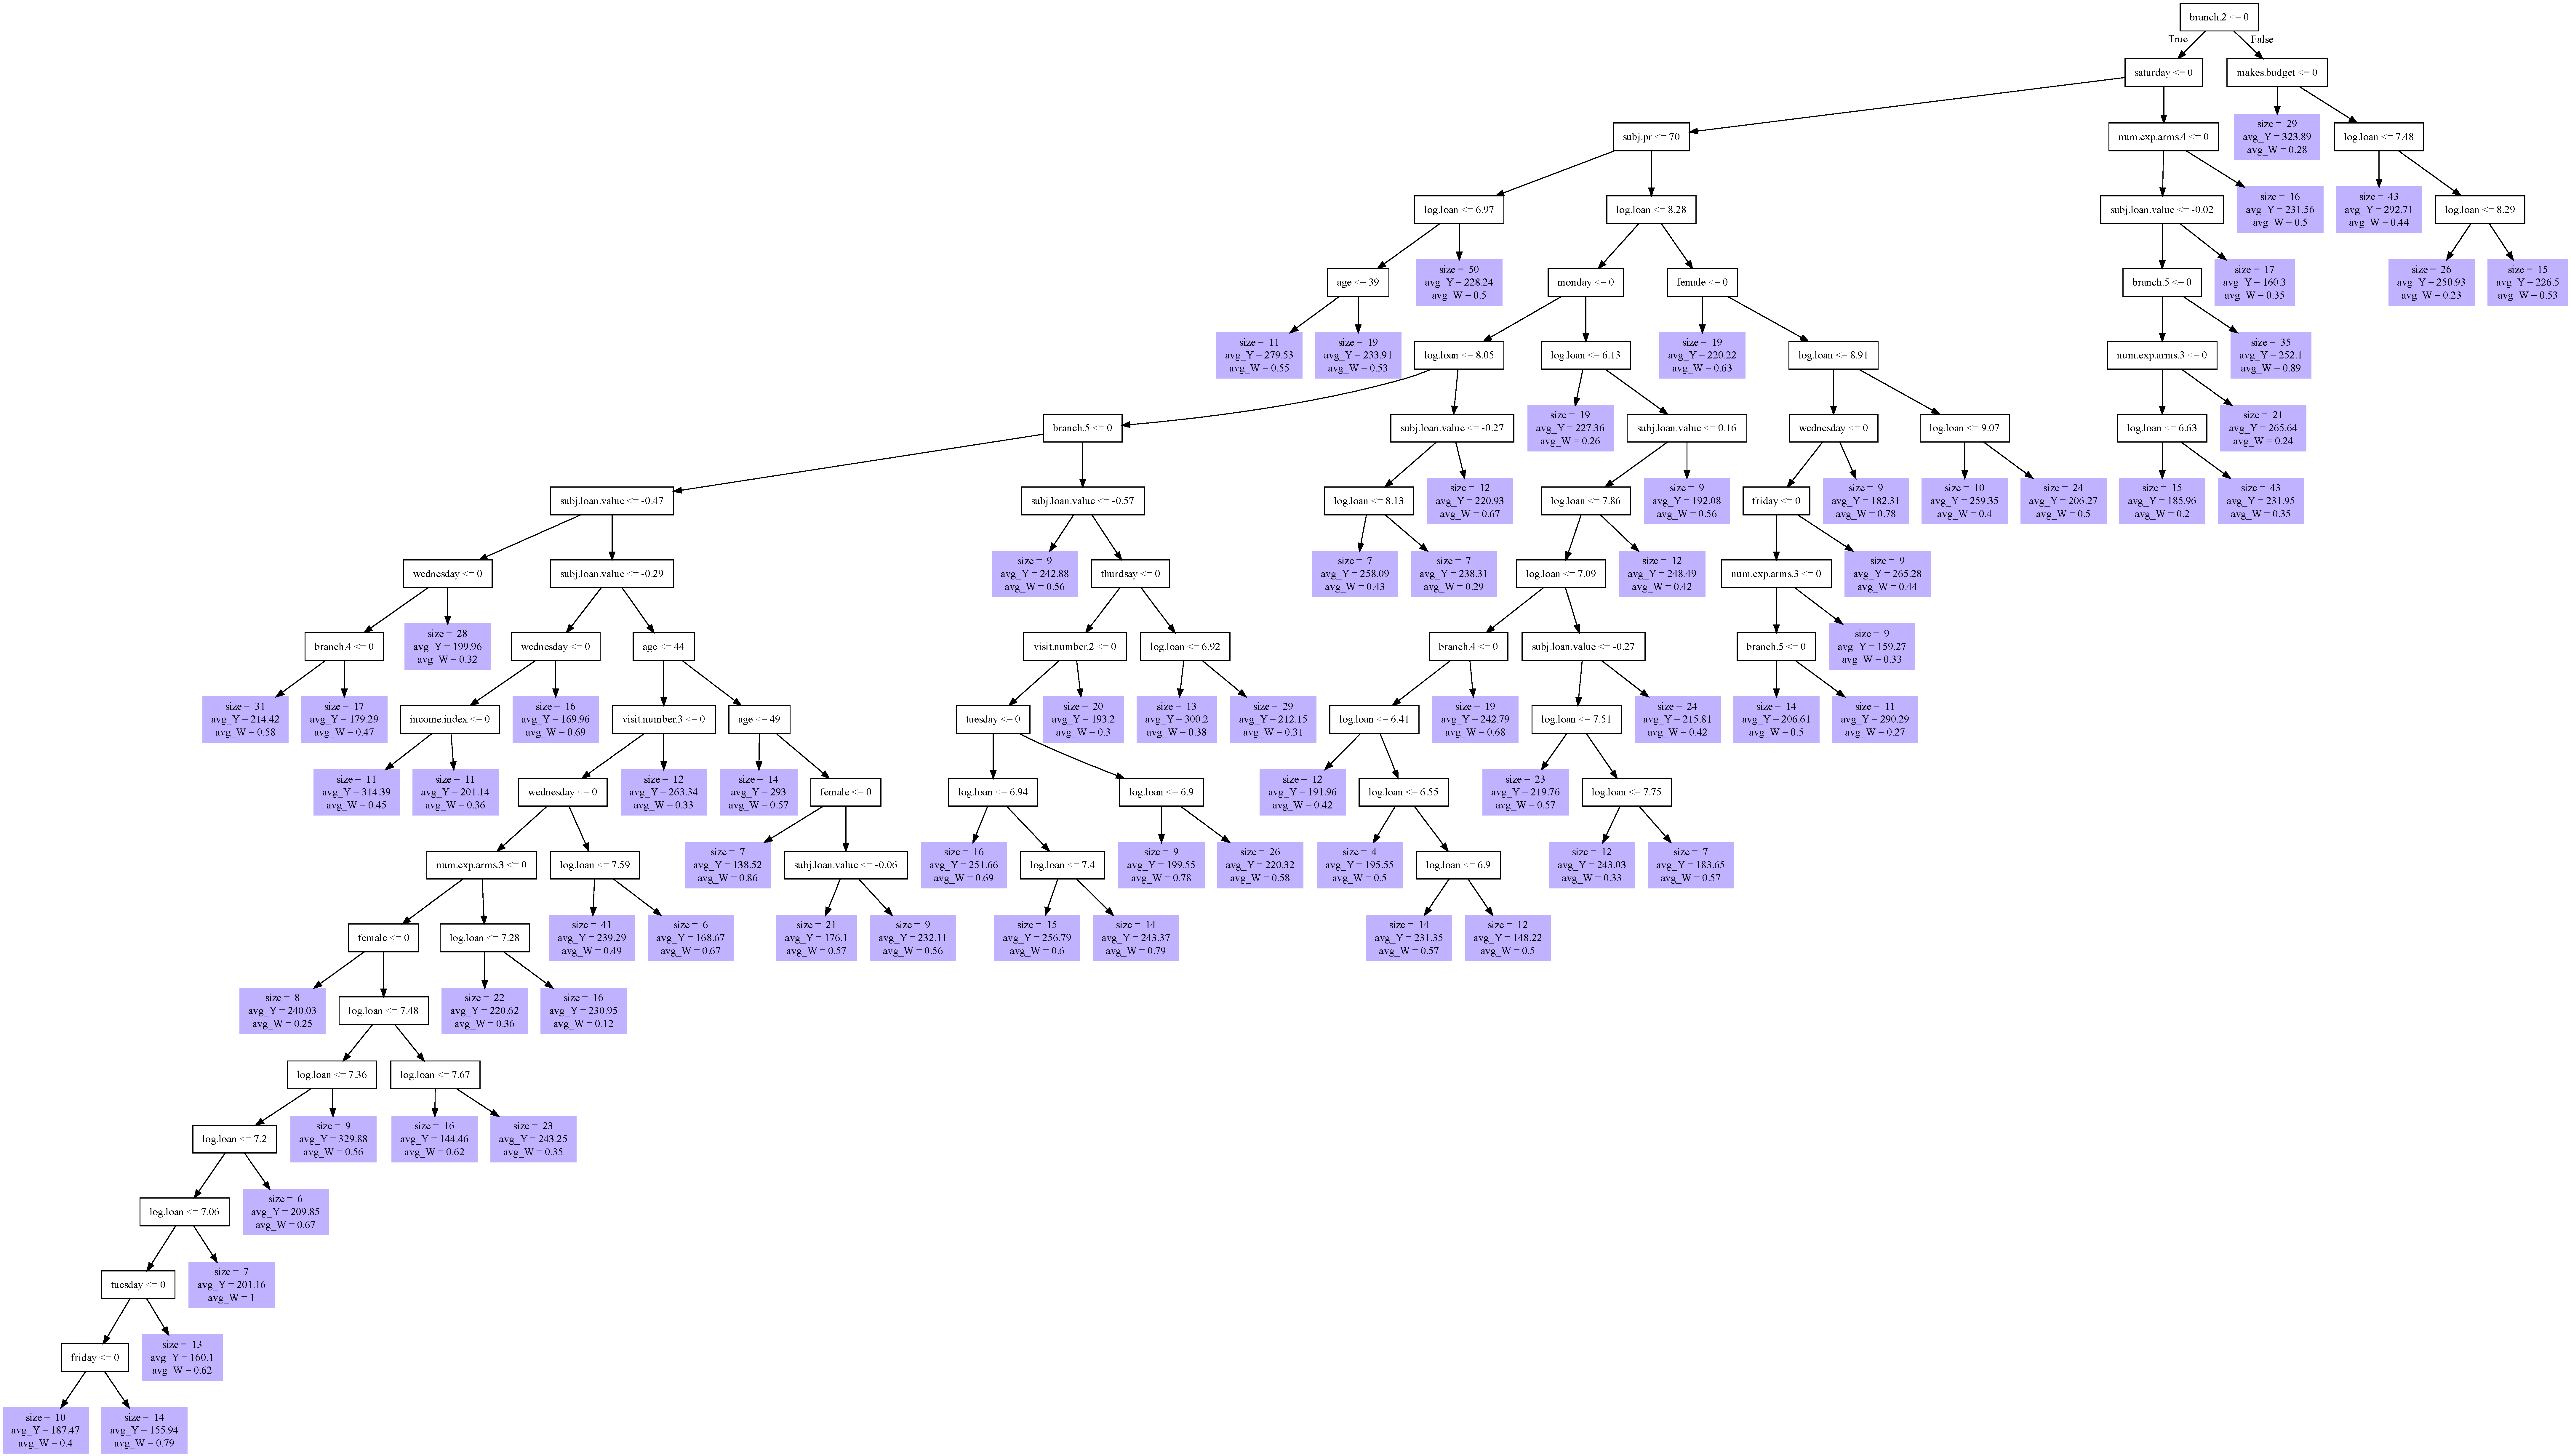
\includegraphics[width=\textwidth]{Figuras/crf_pro_2_apr.pdf}
    \end{center}
    \footnotesize 
    This is one(it is chosen such that it minimizes the pruned cost, that is it is the tree with the smallest root-node impurity) of the honest causal trees in the random forest we use for the estimation of the heterogeneous treatment effect of the fee-forcing contract. It is meant only as an example of how these trees look like. The forest was such that there are as many estimated treatment effects as there are clients.
     %\footnotesize{ \textit{RScript: }  \texttt{grf.R}
\end{figure}

We use \cite{atheygrf} \texttt{causal\_forest} of the \texttt{grf} library in $R$. The parameters used were:
\scriptsize{\textit{causal\_forest(
  X, 
  Y, 
  W, 
  Y.hat = NULL, 
  W.hat = NULL, 
  num.trees = 2000, 
  sample.weights = NULL, 
  clusters = NULL, 
  equalize.cluster.weights = FALSE, 
  sample.fraction = 0.5, 
  mtry = min(ceiling(sqrt(ncol(X)) + 20),ncol(X)), 
  min.node.size = 5, 
  honesty = TRUE, 
  honesty.fraction = 0.5, 
  honesty.prune.leaves = TRUE, 
  alpha = 0.05, 
  imbalance.penalty = 0, 
  stabilize.splits = TRUE, 
  ci.group.size = 2, 
  tune.parameters = "none", 
  tune.num.trees = 200, 
  tune.num.reps = 50, 
  tune.num.draws = 1000, 
  compute.oob.predictions = TRUE, 
  orthog.boosting = FALSE, 
  num.threads = NULL)}}


\begin{figure}[H]
        \caption{Single causal tree for the Forced-commitment contract heterogeneous treatment effects}
    \label{casual_tree}
    \begin{center}
        \centering
        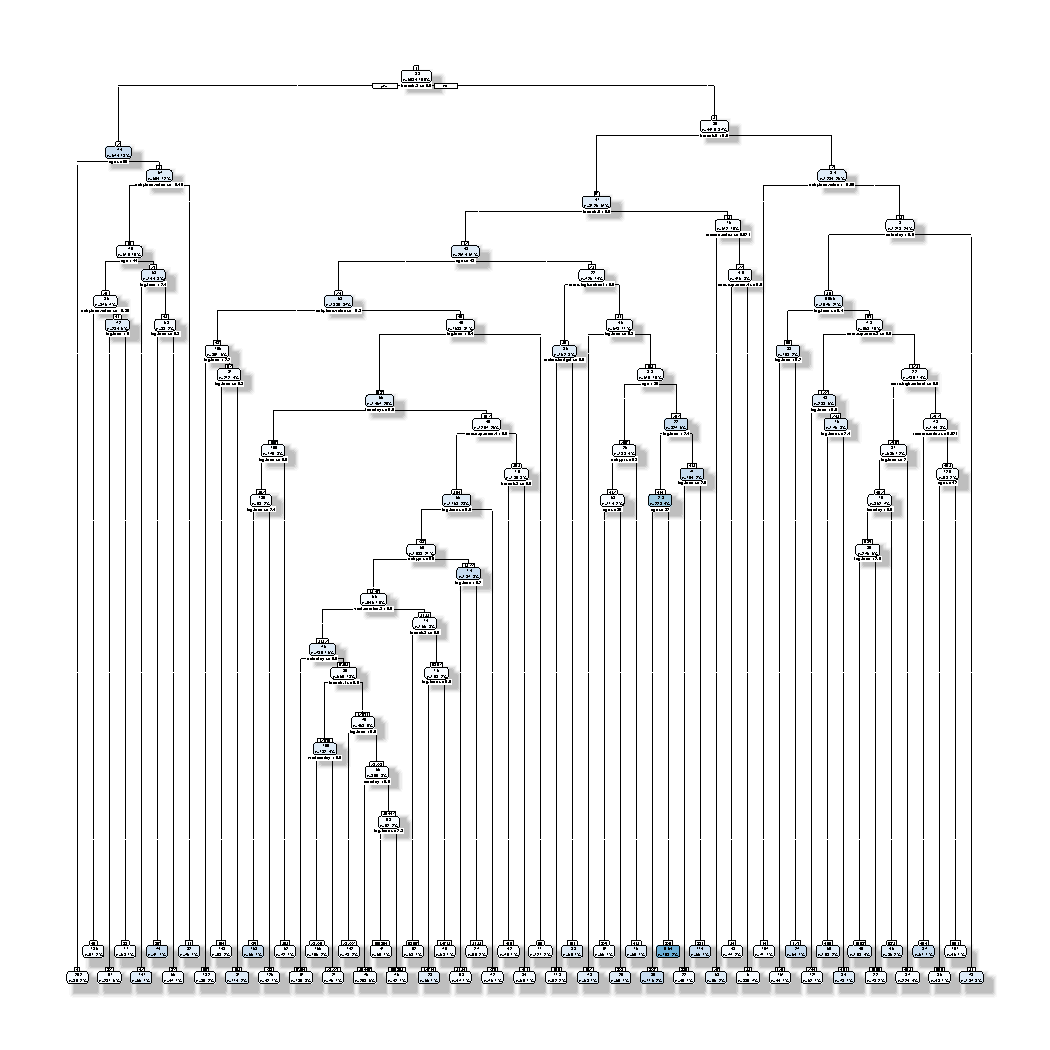
\includegraphics[width=\textwidth]{Figuras/ct_pro_2_apr.pdf}
    \end{center}
    \footnotesize 
   
     %\footnotesize{ \textit{RScript: }  \texttt{grf.R}
\end{figure}





\begin{figure}[H]
    \caption{Choice of contracts and treatment effects}
    \label{choose_wrong}
    \begin{center}
        \begin{subfigure}{0.45\textwidth}
        \caption{Mistakes in choice arm}
        \centering
        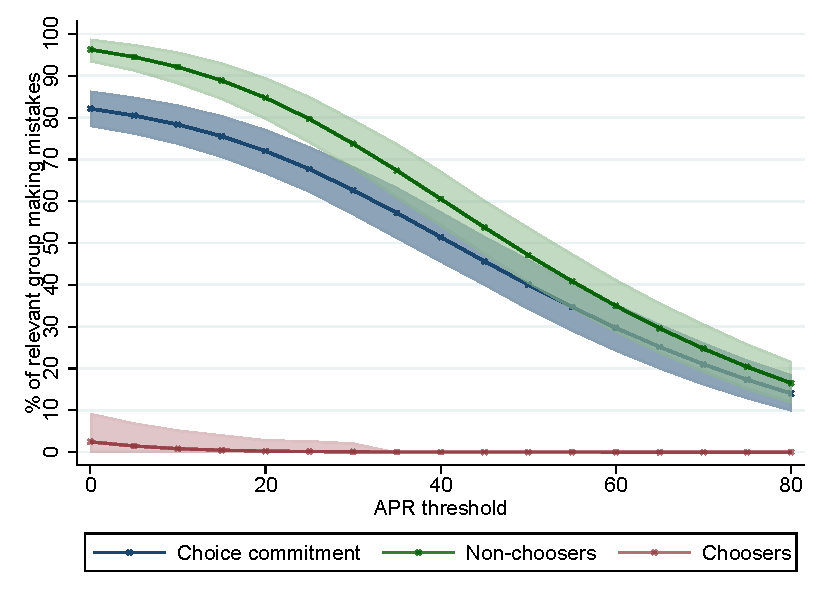
\includegraphics[width=\textwidth]{Figuras/line_cw_apr_te_cf.pdf}
        
    \end{subfigure}
        \begin{subfigure}{0.45\textwidth}
        \caption{Financial value of mistake}
        \centering
        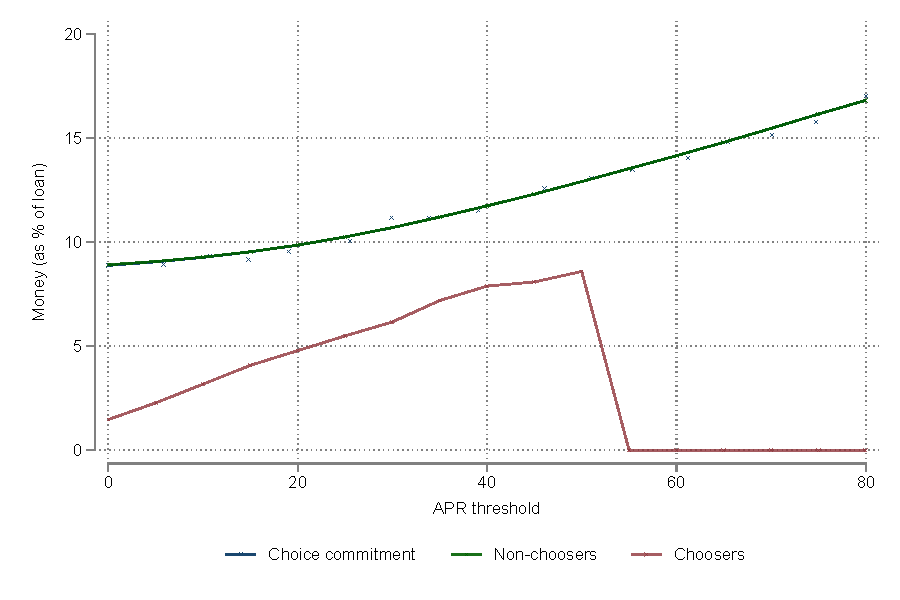
\includegraphics[width=\textwidth]{Figuras/money_cw_apr_te_cf.pdf}

    \bigskip
        
    \end{subfigure}
        \begin{subfigure}{0.45\textwidth}
        \caption{\% better when forced to forced commitment}
        \centering
        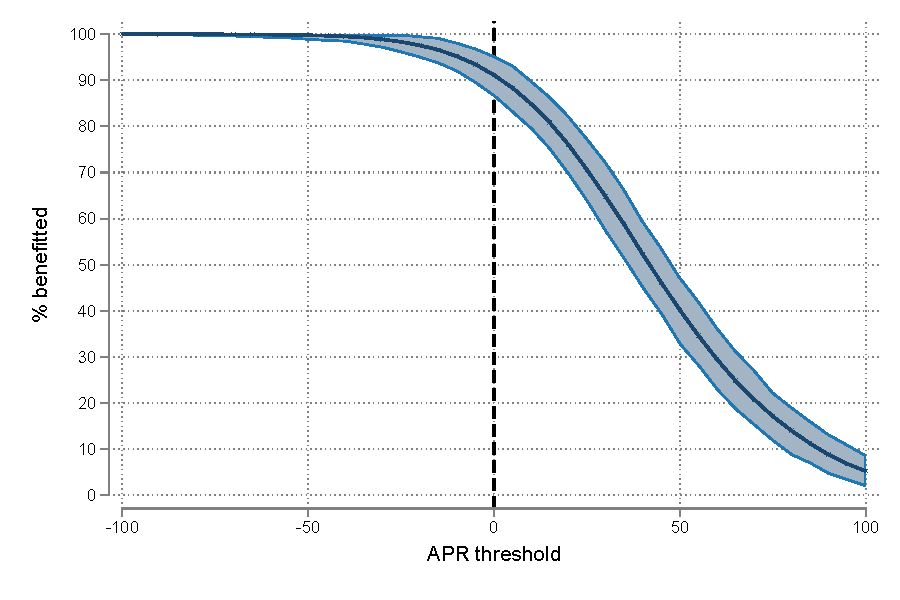
\includegraphics[width=\textwidth]{Figuras/line_better_forceall_apr_te_cf.pdf}
        
    \end{subfigure}
    %     \begin{subfigure}{0.45\textwidth}
    %     \caption{\footnotesize{Effect of CATE benefit vs predicted take-up}}
    %     \centering
    %     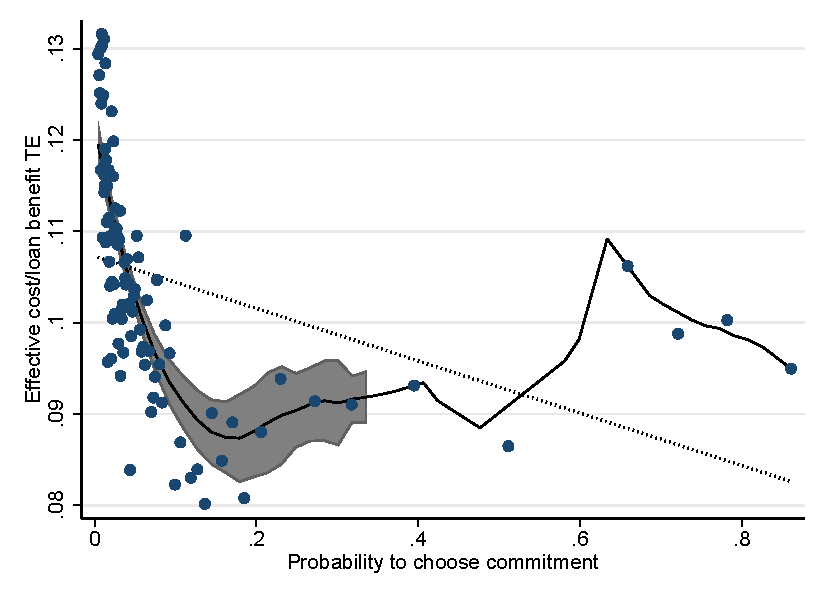
\includegraphics[width=\textwidth]{Figuras/benefit_choice.pdf}% takeuppr_def.pdf 
    % \end{subfigure}
    
    \end{center}
        \scriptsize
        In Panel (a) we estimate what the treatment effect of the commitment contract \textit{would have been} for all subjects in the choice arm if they had been forced into the fee-commitment contract. To do this we proceed in two steps. First, we estimate treatment effects in the forcing arm by comparing the Forced Commitment arm against the status quo arm. We let these effects be heterogeneous as a function of our $x$'s using \cite{atheygrf}'s methodology of causal forests. Second, we extrapolate these treatment effects based on the choice arm using the same $x$'s. Once we have personalized counterfactual treatment effects in the choice arm we calculate what fraction of subjects in the choice arm incurred in financial costs that are  $> z$\% than if they had chosen the opposite contract of what they actually chose, were $z$\% is defined as a fraction of the loan. $z$\% is a level of tolerance we can vary and we plot it in the X-axis. The left Y-axis measures the fraction of subjects that would have been better by a margin of $z$\% if they changed their choice, and the right Y-axis measures the amount of money ``left on the table''. We use bootstrap to tighten the confidence intervals (CIs). \cite{atheygrf}'s heterogeneous treatment effect using GRF is asymptotically normal. We compute the HTE ($\mu$) together with standard errors ($\sigma$) . For every pledge, we draw a random effect from a normal distribution with parameters ($\mu$,$\sigma^2$), and compute via bootstrap the percentage that choose wrong, along normal-approximation CIs (results are robust if we use instead percentile CIs or bias-corrected CIs) . This allows us to estimate a distribution for the upper and lower bound CIs, which we then use to obtain a 95\% CI. Panel (b) is analogous to Panel (a) except that it does the exercise separately for clients we classified as overconfident ($OC_i:=\mathbbm{1}(P^s_i-\widehat{P_i(X_i)}>0))$ and those we classified as not overconfident. Panel (c) simulates what percentage would be better by at least $z$ if we forced everybody of those in the Commitment Choice arm into the fee-commitment contract.
        % Panel (d) asks whether it is the case that people with larger causal benefits from the Forced Commitment contract would be more likely to select that contract. To do this we proceed in two steps as well. First we estimate a flexible model of take-up of the fee commitment contract \textit{in the choice arm} using random forests, and from this model obtain a probability $P(x_i)$ of choosing the Forced Commitment contract for a client with characteristics $x_i$. We extrapolate this model to clients in the Forced Commitment arm to estimate what would they have chosen if we had given them choice. 
        % Figure (d) plots $\widehat{P(x_i)}$ in the X-axis using a binscatter that splits the X-axis in 100 percentile bins. The Y-axis plots the heterogeneous treatment effects of the fee forcing contract on the probability of losing the pawns (more negative means then more likely to recover it), averaged for the respective x-axis bin. Positive assortative selection would mean a negative relationship: those who benefit more by treatment and lose the pawn less are \emph{less} likely to choose it.  Using all bins we estimate a slope of zero in the relationship. Using the 80 right most points, we estimate a \textit{positive} relationship.
        %\textit{Do file: }  \texttt{choose\_wrong\_quant\_wrong.do, choose\_wrong\_quant\_wrong\_decomposition.do}
\end{figure}






\subsection{Take up}


\begin{table}[H]
    \caption{Predicting Take-up: Goodness-of-Fit}
    \label{Table_compliance}
    %\begin{subtable}{1\textwidth}
    % \centering
    %    \caption{Take up}
    %    \scriptsize{% Table generated by Excel2LaTeX from sheet 'oos_pago_frec_vol'
\begin{tabular}{lcccc}
\toprule
      & \multicolumn{4}{c}{Frequent voluntary payment } \\
\midrule
\midrule
OOS measures & Logit & SW-Logit & RF    & Boosting \\
\midrule
\midrule
MAE   & 0.32  & 0.33  & 0.33  & 0.29 \\
MSE   & 0.17  & 0.17  & 0.16  & 0.16 \\
AUC (out of sample) & 0.71  & 0.71  & 0.77  & 0.73 \\
      & (0.04) & (0.04) & (0.04) & (0.04) \\
AUC (in sample) & 0.77  & 0.76  & 0.88  & 0.96 \\
      & (0.02) & (0.02) & (0.01) & (0.01) \\
Accuracy & 0.7   & 0.7   & 0.75  & 0.77 \\
Correlation (0-1) & 0.21  & 0.22  & 0.39  & 0.38 \\
Correlation (predicted val) & 0.33  & 0.33  & 0.42  & 0.4 \\
R-squared  & 0.11  & 0.11  & 0.16  & 0.15 \\
Expected value of predictions & 0.25  & 0.25  & 0.24  & 0.22 \\
\bottomrule
\bottomrule
\end{tabular}%
}
    %\end{subtable}%
    
    %\bigskip
     \begin{subtable}{1\textwidth}
      \centering
        \caption{Take up: Choice-fee Arm}
        \scriptsize{% Table generated by Excel2LaTeX from sheet 'oos_pago_frec_vol_fee'
\begin{tabular}{lcccc}
\toprule
      & \multicolumn{4}{c}{Frequent voluntary payment - FEE} \\
\midrule
\midrule
OOS measures & Logit & SW-Logit & RF    & Boosting \\
\midrule
\midrule
MAE   & 0.21  & 0.21  & 0.23  & 0.17 \\
MSE   & 0.1   & 0.1   & 0.1   & 0.09 \\
AUC (out of sample) & 0.76  & 0.78  & 0.84  & 0.85 \\
      & (0.06) & (0.06) & (0.06) & (0.05) \\
AUC (in sample) & 0.84  & 0.82  & 0.92  & 0.99 \\
      & (0.02) & (0.02) & (0.01) & (0.01) \\
Accuracy & 0.82  & 0.84  & 0.86  & 0.88 \\
Correlation (0-1) & 0.13  & 0.26  & 0.37  & 0.31 \\
Correlation (predicted val) & 0.33  & 0.38  & 0.37  & 0.43 \\
R-squared  & 0.08  & 0.13  & 0.11  & 0.19 \\
Expected value of predictions & 0.17  & 0.17  & 0.16  & 0.12 \\
\bottomrule
\bottomrule
\end{tabular}%
}
    \end{subtable}
    
      \bigskip
    \begin{subtable}{1\textwidth}
      \centering
        \caption{Take up: Choice-promise Arm}
        \scriptsize{% Table generated by Excel2LaTeX from sheet 'oos_pago_frec_vol_promise'
\begin{tabular}{lcccc}
\toprule
      & \multicolumn{4}{c}{Frequent voluntary payment - PROMISE} \\
\midrule
\midrule
OOS measures & Logit & SW-Logit & RF    & Boosting \\
\midrule
\midrule
MAE   & 0.41  & 0.41  & 0.41  & 0.36 \\
MSE   & 0.24  & 0.23  & 0.21  & 0.21 \\
AUC (out of sample) & 0.63  & 0.63  & 0.7   & 0.72 \\
      & (0.06) & (0.06) & (0.06) & (0.06) \\
AUC (in sample) & 0.83  & 0.82  & 0.9   & 0.97 \\
      & (0.02) & (0.02) & (0.01) & (0.01) \\
Accuracy & 0.62  & 0.67  & 0.65  & 0.7 \\
Correlation (0-1) & 0.15  & 0.25  & 0.23  & 0.32 \\
Correlation (predicted val) & 0.22  & 0.21  & 0.3   & 0.35 \\
R-squared  & -0.06 & -0.05 & 0.08  & 0.08 \\
Expected value of predictions & 0.39  & 0.38  & 0.38  & 0.35 \\
\bottomrule
\bottomrule
\end{tabular}%
}
    \end{subtable}
            \scriptsize
           \\
           \\
           \\
    
     %\textit{Scripts: } \texttt{pred\_take\_up.do, pfv\_pred.R}
\end{table}




\vspace{.1in}
\begin{figure}[H]
    \caption{Out of sample ROC curve}
    \label{roc_curve}
    \begin{center}
    \begin{subfigure}{0.45\textwidth}
        \caption{Take-up in Fee Arm}
        \centering
        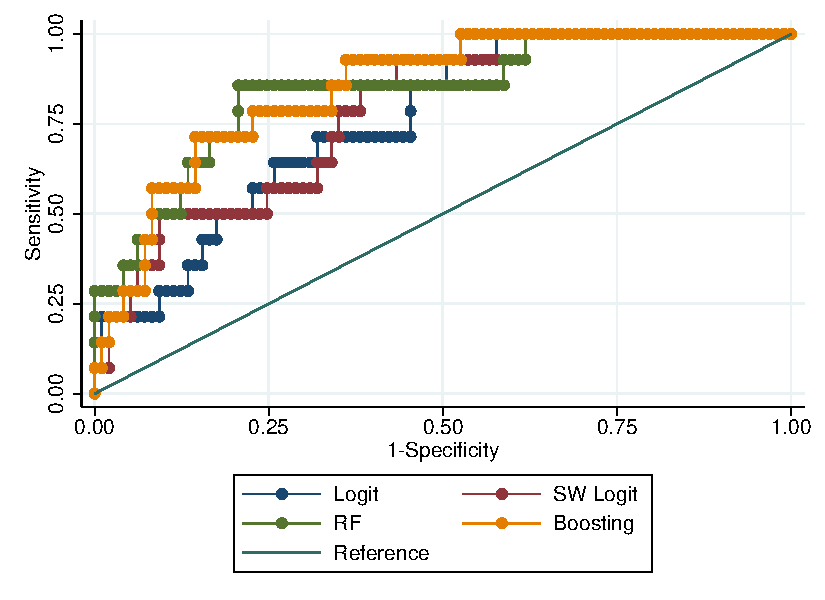
\includegraphics[width=\textwidth]{Figuras/Boost/ROC_curve_outsample_pago_frec_vol_fee.pdf}
    \end{subfigure}
    \begin{subfigure}{0.45\textwidth}
        \caption{Take-up in Promise Arm}
        \centering
        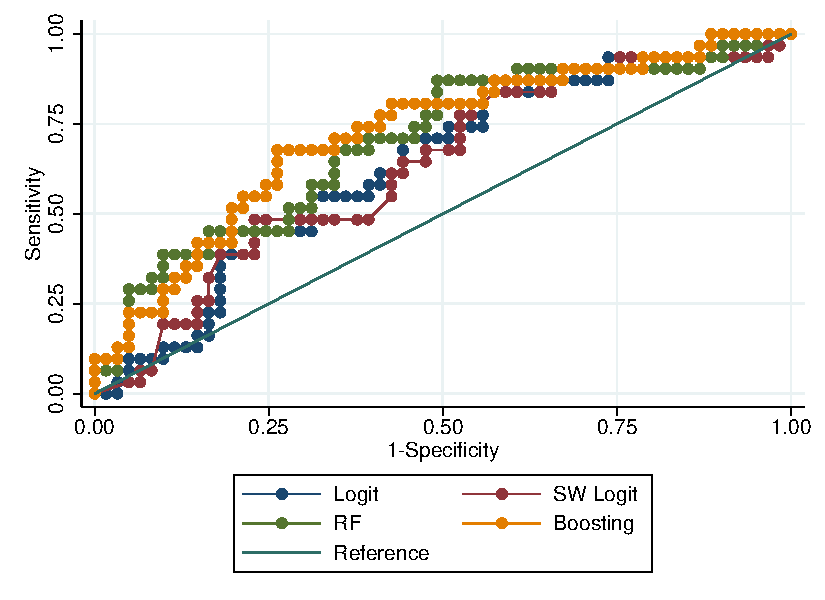
\includegraphics[width=\textwidth]{Figuras/Boost/ROC_curve_outsample_pago_frec_vol_promise.pdf}
    \end{subfigure}
    \end{center}
     \scriptsize 
  %\footnotesize{ \textit{Do file: }  \texttt{pred\_take\_up.do}}
\end{figure}



\begin{figure}[H]
    \caption{Predictors of commitment contract take-up}
    \label{interactions_takeup}
    \begin{center}
    \begin{subfigure}{0.45\textwidth}
        \caption{with Fee Arm}
        \centering
        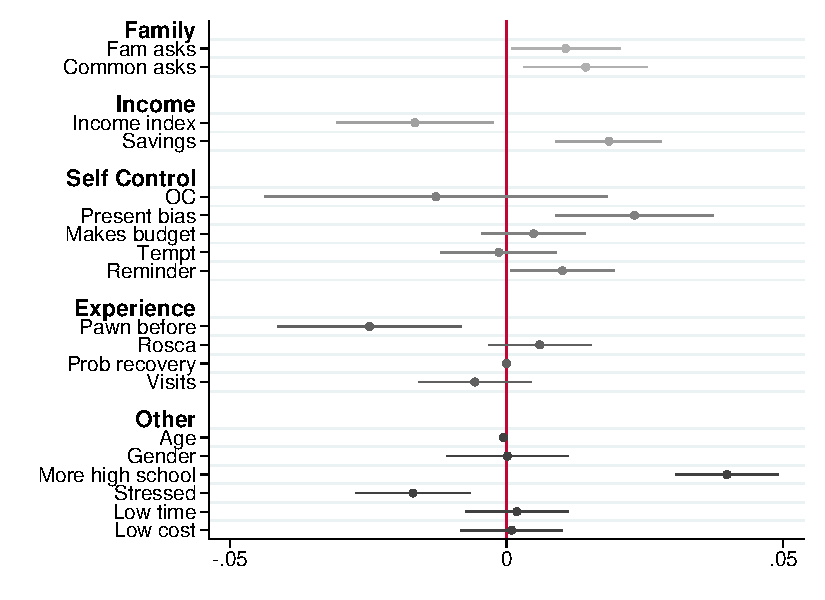
\includegraphics[width=\textwidth]{Figuras/pago_frec_vol_fee_interactions_rf.pdf}
    \end{subfigure}
    \begin{subfigure}{0.45\textwidth}
        \caption{with Promise Arm}
        \centering
        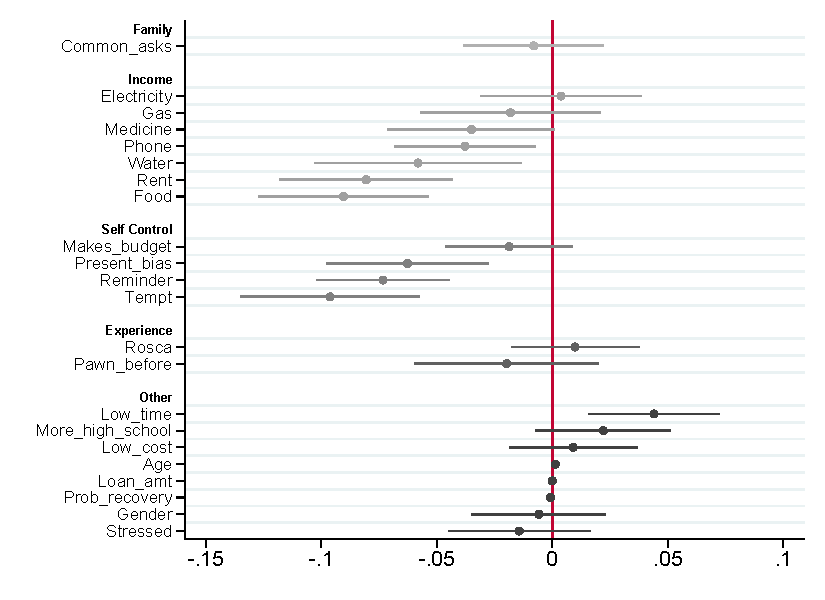
\includegraphics[width=\textwidth]{Figuras/pago_frec_vol_promise_interactions_rf.pdf}
    \end{subfigure}
    \end{center}
     \scriptsize
      %\footnotesize{ \textit{Do file: }  \texttt{analyze\_fvp.do}}
\end{figure}


\scriptsize 
\noindent This figure reports bivariate regressions of the form $\widehat{TakeUp} = \alpha + \beta \: X_i + \epsilon_i$, where $\widehat{TakeUp}$ is the prediction using random forests. The figure reports the $\beta$ coefficients for different $X_i$'s along with 95\% confidence intervals. Panel (a) focuses on take up in the arm where clients could chose among the fee-commitment contract and the status quo contract. Panel (b) focuses on the arm where clients could chose among the promise-commitment contract and the status quo contract. Using random forests we can predict who takes up the fee-forcing contract with 85\% accuracy out of sample.\footnote{Correcting for the fact that most chose the status-quo contract using the method of SMOTE, \cite{smote} we find an accuracy rate of 75\%.} Which suggests that choice among contracts is not purely random. This figure shows that the more educated, those that report that their family typically asks for money, those that make a monthly budget of expenses, and those that ask for a remainder of their due payments (and marginally those we classify as present-biased) are more likely to chose the fee-commitment contract if given the choice. The opposite holds for clients that are more economically vulnerable (can barely pay for food, electricity, etc) and those that report being more stressed.



\subsection{Selection on gains}


\begin{figure}[H]
    \caption{Determinants of treatment effects and probability of choosing commitment}
    \label{determinants_ps_hte}
    \begin{center}
    \begin{subfigure}{0.475\textwidth}
        \caption{Determinants of HTE}
        \centering
        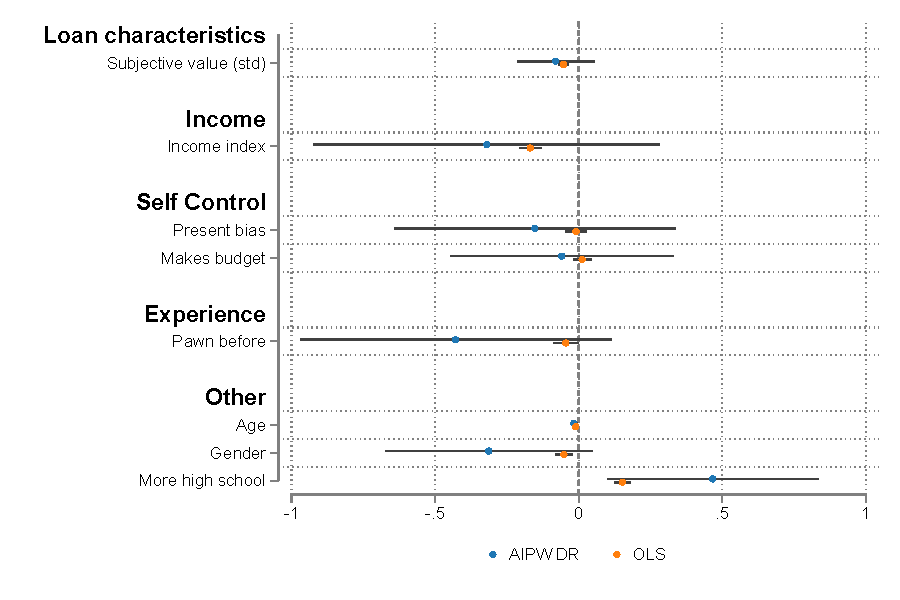
\includegraphics[width=\textwidth]{Figuras/HE/he_int_vertical_apr_pro_2.pdf}
    \end{subfigure}
    \begin{subfigure}{0.475\textwidth}
        \caption{Determinants of propensity score}
        \centering
        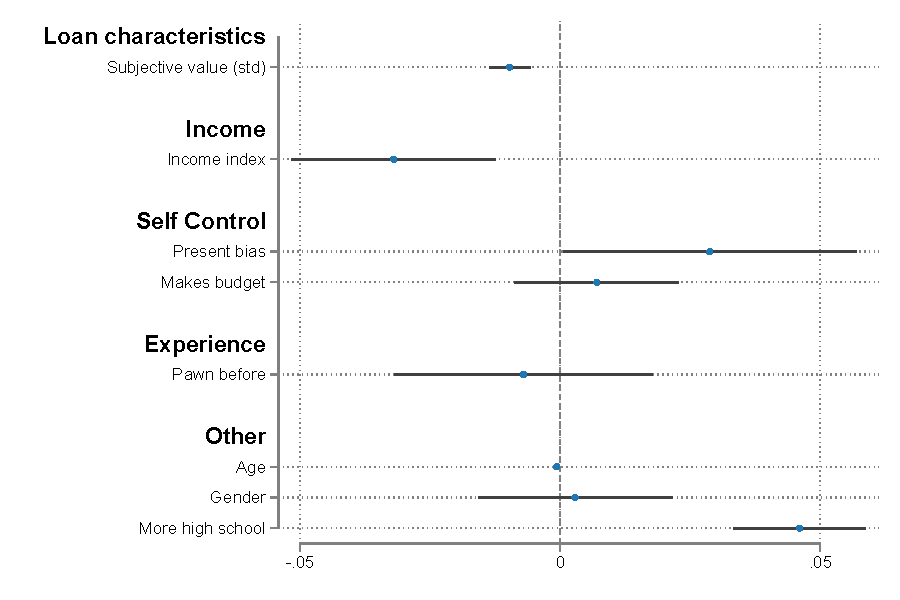
\includegraphics[width=\textwidth]{Figuras/HE/ps_int_vertical_pr_gbc_1.pdf}
    \end{subfigure}
  
    \end{center}
     \scriptsize   This figure estimates bivariate regressions of the estimated client-level (a) heterogeneous treatment effects, (b) propensity score, against the respective covariate from the baseline survey  $\widehat{HTE_i}, \widehat{P_i} = \alpha + \beta \: X_i + \epsilon_i$. The regressors $X_i$ include (e.g if the family asks for money, if they have savings, if they are overconfident using the definition the text, etc. See this Appendix for a transcription of the survey). \\
      %\footnotesize{ \textit{Do file: }  \texttt{analyze\_grf\_single\_arm.do}} \texttt{benefit\_choice.do}}
\end{figure}



%%%%%%%%%%%%%%%%%%%%%%%%%%%%%%%%%%%%%%%%%%%%%%%
%%%%%%%%%%%%%%%%%%%%%%%%%%%%%%%%%%%%%%%%%%%%%%

% APPENDIX B


\section{Mechanisms }


\subsection{Optimism, Over-Optimism, and the Failure of Self-Commitment}
\label{overconfidence}

\textcolor{red}{Need to decide whether we want to try to plant our feet on Confidence/Overconfidence as the core `why' of the previous result
.}
%\subsubsection{Behavioral: overconfident borrowers demand less (but benefit more)} \label{behavioral}

The leading behavioral explanation in the literature for low demand for commitment is present biased preferences with naivete (e.g. \cite{Rabin2018}, \cite{John}, \cite{Laibson2018})  \cite{Laibson2015} shows that the lost flexibility resulting from a commitment contract can limit take-up especially severely when agents are (partially) naive about their self control problem. In our context if consumers are (partially) naive about their present bias, they would plan to save more (or spend less) than what they actually end up saving, thus making it be harder to recover their pawn. This under-saving will be mitigated in the fee forcing contract since the fee makes them save money to pay part of the loan periodically. \ref{appendix_c} formalizes this in a model. Another behavioral explanation is that clients may underestimate the likelihood and severity of negative income shocks. Both of these explanations predict that clients will be overconfident about their likelihood of pawn recovery. Recall that in the control group the client's subjective probability of recovery is on average 93\%, while actual recovery is just 44\%. A further piece of evidence consistent with underestimating negative income shocks and with present bias with partial naivete is that a large number of people (25\%) in the control group pay a positive amount toward pawn recovery but end up losing their pawn anyway.


So, overconfidence of recovering the pawn is implied by both present bias preferences with naivete and upward bias in their income expectations. But does overconfidence actually predict low demand for commitment empirically? It does. We define as overconfidence as the reported subjective probability of recovery minus the predicted probability based on the client's characteristics, $P^s_i-\widehat{P_i(X_i)}$.\footnote{We predict $\widehat{P_i(X_i)}$ in two steps. In step one we use Lasso with cross validation to tune the regularization parameter to select the most predictive variables $X$. The typical present bias question as in \cite{Ashraf} was eliminated in this step. In the second step we estimate $\widehat{P_i(X_i)}$ using those variables in a logit model. The Lasso selected variables were type of pawn, female, age, has pawned before, has savings, participates in rotating savings, often feels tempted to change plans, would like to have a reminder to pay, and an economic vulnerability index. We are careful not to include these variables as controls in Table  \ref{oc_reg}.} There is a large amount of overconfidence in our context. Figure \ref{oc_hist} plots a histogram of $OC_i$ and shows that the overwhelming majority display overconfidence, and a large fraction overestimate recovery by more than 50 percentage points. Our measure of overconfidence is useful especially when there is limited time for a detailed survey.\footnote{It may be more useful than a simple elicitation of present bias as in \cite{Ashraf}. We find that 15\% of clients are classified as present biased using this measure of preference reversal. This level is similar to the number \cite{Ashraf} find but small to explain no take-up of commitment for 90\% of clients. This measure was not correlated with take up of commitment in our sample.} First it is very prevalent, which makes it promising to explain the overwhelming prevalence of low take up. Second, it is easy to measure. Third, it is predictive of take-up in an intuitive way. Finally, overconfidence in recovery is implied by present bias with (partial) naivete but also by biased expectations of negative income shocks, thus capturing both kinds of bias.\footnote{\textcolor{red}{Another indication of overconfidence is that in our data, of those who renew, 83\% lose the pawn anyway. Our measure of overconfidence has a correlation of \hl{xxx}\% with a dummy for renewing and losing the pawn. }} 

\cite{Sprenger} have argued that it is critical to understand the link between beliefs and demand for commitment, yet the evidence is scarce. Table \ref{oc_reg} does this: it regresses an indicator of take up of the monthly payment contract against an indicator for overconfidence $OC_i:=\mathbbm{1}(P^s_i-\widehat{P_i(X_i)}>0)$ and controls. Controls $Z$ include branch and day of the week dummies, schooling, whether the client does a monthly budget plan, among others. We are careful not to include controls that were used in $\widehat{P_i(X_i)}$. % and a measure of intertemporal preference reversal analogous to that of \cite{Ashraf} as controls.\
In the choice-fee arm, being overconfident decreases the likelihood of demanding commitment by 12 percentage points a result that this is robust to including controls  (columns 1 and 2). While overconfidence predicts lower take up in the Commitment Choice arm, this is not the case in the promise-choice arm (columns 3 and 4).  One interpretation of the results is that the overconfident borrowers think they do not need commitment, and their demand decreases sharply as soon as there is even a small fee, and at the same time they perceive the promise as a low cost option. This provides evidence for \cite{Sprenger}'s conjecture that ``tepid demand for commitment outside controlled experimental settings is consistent with broad unawareness [of biases]''. 

How does overconfidence map to cost outcomes? Theory predicts that the more overconfident (naive) may be at the same time those that benefit more from commitment. Extrapolating individual treatment effects of the Forced Commitment contract vs the status quo one to the choice arm (see below for more detail), and using them as a dependent variable we find that overconfident borrowers benefit \textit{more} from the commitment contract, with {24.8}\% (=\${30}/\${121}) more savings (columns 5 and 6). Thus while we predict the overconfident benefit more from commitment, they demand less of it. 




\subsubsection{Neoclassical Alternatives} \label{neoclasical}

\vspace{.1in}
\noindent \textbf{Risk aversion.} We do not have measures of risk aversion in our short survey, which makes it hard to assess the hypothesis that risk aversion limits take-up of the fee frequent payment contract. One way to proceed is to take the empirical distribution of financing cost ---$F_{fee}(FC)$--- as one the client would have faced had she chosen the the fee-commitment contract. We could then ask what would risk aversion have to be in order to justify the client choosing the fee-commitment contract distribution of costs over the distribution associated with the status quo contract, $F_{sq}(FC)$. Framed as a choice among cost distributions, we can calculate what risk aversion is needed to rationalize the overwhelming choice of the status quo contract over the fee-commitment contract. This exercise of course assumes --as is common in economics-- that clients know the distribution of financial cost, that the distribution is common across consumers (although this can be relaxed), and that this cost distribution is the only difference among contracts. 

Fortunately for us, it turns out that one distribution first-order-stochastically dominates the other, obviating the need to calibrate a specific utility function or use a parametric distribution function in order to rank them in terms of expected utility. We use the fact that if the utility $u(FC)$ is decreasing in $FC$ (i.e. clients dislike paying higher financing cost) and $F_{fee}(FC) \geq F_{sq}(FC)$ for all $FC$, which we actually verify in our data, then $E_{fee}[u(FC)] \geq E_{sq}[u(FC)]$, that is any expected utility maximizing client risk averse consumer should choose the Forced Commitment contract as a result of the distribution of cost payoffs.\footnote{See the Appendix for the proof. Figure \ref{ecdf_fc} in the Appendix shows that indeed $F_{fee}(FC) \geq F_{sq}(FC)$. Table \ref{stochastic_dominance} shows that this holds also for sub-populations of different characteristics.}. Thus, risk aversion cannot explain the low demand for commitment under the assumptions of this exercise.   


\vspace{.1in}
\noindent \textbf{Lost flexibility.} A second explanation for low take up is lost flexibility. That is, the fee-commitment contract may provide too much commitment which is costly because the client may be forced to incur in late payment fees if he experiences a negative income shock.\footnote{Note that income shocks that affect the ability to pay the entire loan are a worry for both the Forced Commitment contract and the status quo one, and should not make one contract more favorable than the other.} While we cannot rule out that income shocks combined with lost flexibility of the contract explain the low demand, we think it is unlikely. First, we showed above that clients report a subjective probability of recovery of 93\% on average, which suggests they are not too worried about income shocks. Second, the fear of incurring fees is quantitatively not enough of a concern when compared to the savings they are experiencing. %Note that fees for late payment are not that high. In an average loan of 2,000 pesos the monthly payment is close to 700 pesos, and a fee of 2\% of that is 14 pesos (less than \$1 dollar). This is about gr{1\%} of monthly per capita income of the first 3 deciles of Mexican {household's} income distribution. %This compares favorably to the gr{\$11.6 + \$62.3)} pesos transportation / transaction cost of one. 

To make this concrete, we calculated what the financing cost of the fee-commitment contract would be if \textit{all} its clients incurred in \textit{all} potential fees (while keeping payment profiles and pawn recovery constant) and added these fictitious fees to financing cost for those in the Forced Commitment arm, thus artificially inflating their cost. We then re-estimated the quantile treatment effects analogous to Figure \ref{fc_pro2}(b) with this inflated financial cost. %\footnote{Of course behavior may not be constant, but we believe this is a reasonable fist approximation. %It could be that having this small fee added to the balance discourages them to pay or makes it harder to pay back the loan. But the contrary may also happen, with the fee making them more determined to pay early. We would need a structural model of client behavior to estimate a full counterfactual. We suspect that such small fees would not generate large changes in behavior in a simple neoclassical model.}). 
Figure \ref{fc_allfee} presents the results. We find that even in this extreme scenario, tilted against the Forced Commitment contract, the estimated effect still implies cost savings from the Forced Commitment contract at the mean, 25$^{th}$, 50$^{th}$, and 75$^{th}$ percentiles.\footnote{Recall that the differences in financing cost already takes into account the fact that clients in the fee forcing contract sink more pre-payments than those in the status quo contract, and that those prepayments are lost if the loan is not fully paid back.}  Although these arguments are not definitive, they suggest that low demand for commitment may be driven by more than the anticipation of lost flexibility implied by a small fee.

\vspace{.1in}
\noindent \textbf{High time discounting.} We mentioned above that clients in the status quo contract tend to wait until the last moment to pay to recover their pawns. Even among those that recover their pawn, only 40\% pay before the 90$^{th}$ day. Table \ref{mechanisms} shows that clients assigned to the fee-commitment contract front load their payments, starting their first payment earlier and finishing paying earlier too. However, clients may dislike front loading payments if their time preference discount rate is high. They may be willing to trade off a higher probability of losing their pawn for more \textit{back} loaded payments.  

What would discount rates have to be in order for back loaded payments to offset the reductions in financial cost effects we observe? %We can calculate this number by looping across a grid of discount rates, incorporating this higher discount rate in the definition of financial cost, and reestimating equation \ref{basic_reg} with this modified financial cost measure as the dependent variable in equation 1, searching for the discount rate that makes $\beta$ equal zero. We did this and obtained 
We calculate that the discount rate that is necessary to compensate for the savings in financial cost (i.e. that makes the estimated $\beta$ in equation \ref{basic_reg} equal to zero when financing cost --using different $r$'s-- is the dependent variable) is a staggering 8,190 percent per year. We find this discount rate implausibly high even for this credit constrained population\footnote{For comparison, \cite{Levin} find that a discount rate of 1,415 per year for subprime borrowers in the US is too high to be believable.}, casting doubt on high discount rates as explanation for low demand for commitment. %\footnote{In the baseline survey we give respondents a hypothetical choice between $100$ pesos tomorrow or $150$ pesos in one month (an implicit yearly interest rate of {12,800\%}) and only 30\% chose the later one.} 


%%%%%%%%%%%%%%%%%%%%%%%%%%%%%%%%%%%%%%%%%%%%%%%%%%%%%%%%%%%%%%%%%%%%%%%%%%%%%%
%%%%%%%%%%%%%%%%%%%%%%%%%%%%%%%%%%%%%%%%%%%%%%%%%%%%%%%%%%%%%%%%

% APPENDIX C

\newpage
\section{ A simple model}
\label{appendix_c}
\vspace{.2in}
\normalsize
\linespread{1.25}

Although the empirical results are striking and stand alone, this section refers to the model of \cite{John} to interpret our empirical results. The model is stylized but incorporates important features of our context. It allows for negative income shocks which we think are prevalent in this population. %The shock generates a cost of committing to monthly payments and could potentially be a reason for low take up. 
It also features clients with present biased time preferences --allowing for partial naivete-- choosing to save to pay for an expense, and with the opportunity to make a commitment to save and pay. These two features parsimoniously explain several facts about the context --like overconfidence in recovering the pawn--, and about the results --e.g. that forcing commitment seems to help. We intend the model only as a very stylized approximation to our context, and we use it only to help us organize the interpretation of the empirical results, not as a literal description of reality. %Third, it allows for a simple way to model commitment afforded by late payment fees. %Nonetheless, the model abstracts from several details of the context. Even with these abstraction it allows us to explain our six main results listed in Section \ref{explanations_recap} below.

We use the model of \cite{John} and refer the reader to that paper for more detail, justification of assumptions and some of the proofs. The model has three periods and linear utility.\footnote{This does not map perfectly to our 3 period contract, but it is enough to generate the results we need. We also assume that the amount of the loan is used up to pay for the emergency. \cite{John_theory} provides a more general treatment.} Period $t=0$ is a planning period where the client is either allocated to the status quo, the fee-forcing contract, or a choice between the two. Period $t=1$ is the saving-for-the-monthly-payment  period, and $t=2$ in the pawn recovery (loan payment) period. In period 1 the client receives her income $y_1=1$, or gets zero with probability $\lambda$. She can consume ($c_1$) or save ($s_1$) part that income. In period 2 the client gets her savings from period 1, and again receives income of either $y_2=1$, or zero with independent probability $\lambda$. In this last period, she decides whether to use income and savings for consumption $c_2$ and/or for paying back the loan of size $p \in(1,2)$ to recover the pawned piece valued at $b>p$. In this simple set up we model the fee-commitment contract as a contract that imposes a fee of size $F$ if the client fails at $t=1$ to save $s_1=p-1$ pesos, which is what is needed to pay the loan back when there are no shocks. In period $t=0$ she evaluates her welfare as $E[c_1+c_2]$, were for simplicity we have set the time discount to one. We also assume the interest rate is one. We introduce present biased preferences by assuming the following utility function $U_t=c_t+\beta \: \sum_{k=t+1}^{2} E[c_k]$, with $\beta<1$ indicating present bias. A naive client perceives she is not so present biased and instead of $\beta$ uses $\hat{\beta} \in (\beta,1]$. 

Note that under these assumptions it is efficient at $t=0$ to recover the loan since $b>p$ and since there is no discounting at $t=0$. Because $b>1$, paying back the loan requires that there is no negative shock in any period and that $s_1>0$. Because $\beta<1$ at $t=1$ the client will not send savings in excess of what is needed to recover the loan: $s_1=p-1$. This parsimonious model implies the following results:

\vspace{.2in}
\noindent \textbf{Result 1: Present biased clients default more.} Under the status-quo contract, absent shock realizations, present biased clients (sophisticated or naive) with $\beta<\beta_{SQ}<1$ will lose their pawn, while clients with no present bias will not.\footnote{$\beta_{SQ}=\frac{p-1}{\lambda(p-1)+(1-\lambda)(b-1)}$. See Proposition 1 in \cite{John}.} 

\vspace{.1in}
\noindent \textbf{Result 2: Forcing present-biased clients into the fee-commitment contract reduces default.} Imposing a fee $F>0$ for late payments weakly decreases default (for present biased clients only). It strictly decreases default if $F>F_{min}(\beta):=(p-1)-\beta[\lambda(p-1)+(1-\lambda)(b-1)]$. The larger the present bias the larger the $F$ required to induce pawn recovery.\footnote{$F_{min}(\beta)$ is derived from the incentive compatibility constraint needed to generate savings at $t=1$ to recover the pawn can be written as $1-(p-1)+\beta[\lambda(p-1)+(1-\lambda)(b-1)] \geq 1-F+\beta(1-\lambda)$.}

\vspace{.1in}
\noindent \textbf{Result 3: Demand for commitment.} Given $F>0$, (a) Neoclassical clients will never demand commitment. (b) Present-biased sophisticated clients will prefer the fee-forcing contract over the status quo contract $\iff$  $\lambda \: F<(1-\lambda)^2(b-p)$ and $F>F_{min}(\beta)$, that is $\iff$  $\beta \in [\beta_{min},\beta_{SQ}]$.\footnote{$\beta_{SQ}$ was determined in Result 1. $\beta_{min}$ is such that $F=F_{min}(\beta_{min})$.} (c) Analogously, naive clients will demand commitment $\iff$ $\hat{\beta} \in [\widehat{\beta_{min}},\beta_{SQ}]$, where $\widehat{\beta_{min}}<\beta_{min}$. So strongly naive clients will on the one hand demand more commitment than sophisticated clients since they believe (incorrectly) that a smaller fee will motivate them to pay. On the other hand they may demand less commitment since they think they can save and pay on their own. Whether they demand more or less than sophisticated clients depends on the empirical distribution of $\beta$ and $\hat{\beta}$. 

\vspace{.1in}
\noindent \textbf{Result 4: Overconfidence.} Only naive clients will be overconfident about the probability of recovery. This will be true whether they have the status quo or the fee-forcing contract. Overconfidence is increasing in $\hat{\beta}$.

\vspace{.1in}
\noindent \textbf{Result 5: Welfare.} (a) Neoclassical consumers' welfare strictly decreases when we force clients into the fee-commitment contract instead of the status quo contract because of the risk of them not being able to pay for the installment, and does not change when we offer a choice between them. (b) The welfare of sophisticated present biased consumers weakly increases when we give them choice, and it strictly increases  $\iff$  $\beta \in [\beta_{min},\beta_{SQ}]$, that is when they would choose the fee-commitment contract themselves. Forcing them into the fee-commitment contract increases welfare $\iff$  $\beta \in [\beta_{min},\beta_{SQ}]$, otherwise it strictly decreases it. So choice is better than forcing for sophisticates. (c) Forcing can be welfare improving for the naive. Indeed if $\hat{\beta}>\beta_{SQ}>\beta$ then forcing the fee-commitment contract increases welfare, and if $\hat{\beta} \in (\widehat{\beta_{min}},\beta_{min})$ then forcing the status quo contract increases welfare.\footnote{This result is different from that in \cite{John}. Her context has individuals choosing the size of the fee. In that context naive clients will \textit{always} chose the wrong fee size and default later, therefore choice is always decreasing for the naive. In our context $F$ is fixed at 2\% of the balance due, and this implies that choice could be welfare improving for some naifs.} We want to highlight that only under certain parameters will forcing installment payments improve welfare, and that welfare will likely decrease for those with no present bias and the sophisticated present biased consumers. 

\vspace{.1in}
\noindent \textbf{Result 6: Welfare and ex-post observed behavior.} If for a naive client $i$ the fee-forcing contract causes higher pawn recovery, then we know the fee $F$ made her IC constraint binding, and therefore that $\hat{\beta}_i>\widehat{\beta}_{min}$. If in addition if it was the case that $\beta_i<\beta_{SQ}$. %\footnote{\hl{Isaac, aqui tengo dos pregutas: (1) si es $\beta$ y no $\hat{\beta}$ verdad?  (2) Para que una persona naive empenie en el status quo tiene que ser que cree que va a recuperar no? Es decir tiene que ser $\hat{\beta}>\beta_{SQ}$ correcto?}} 
then the fee-forcing contract would have increased welfare for the naive. That is, our finding that the fee-forcing contract increases pawn recovery is a sign of higher welfare (although not a sufficient condition).\footnote{It is not sufficient since ex-ante the commitment $F$ may have been too expensive given the income shocks, i.e. if $\lambda \: F>(1-\lambda)^2(b-p)$.}




\subsection{Interpretation}

The model is very parsimonious but powerful and it can potentially explain all our empirical findings qualitatively.\footnote{The model is sufficiently stylized that we think we would not gain much from estimating it. Furthermore we have no data on income shocks which figure prominently in the model. \cite{Ted} and \cite{Aprajit} are two very recent models that combine a field experiment with commitment contracts and estimation of present bias parameters.} First, it can explain why default is high in the status-quo contract, namely that clients are present biased and have no commitment devices. Second, it can explain why clients are overconfident in our data, namely by virtue of naivete about present bias. Under the model naivete is necessary to explain this. Third, it can also explain why the fee forcing contract induces lower default, but not for everyone: namely that it makes the incentive compatibility constraint for payment binding for the present biased, while it was not binding in the status quo contract. Fourth, it can also explain why there is low demand for commitment even if it seems to improve welfare: namely that there is a small share of neoclassical and sophisticated clients, and at the same time naifs have a present biased parameters values in the region in which they think they can save on their own. Fifth, it explains non-zero demand for commitment for a set of clients. Sixth, it can explain why clients exposed to the Forced Commitment contract are more likely to come back namely those naifs whose welfare increased as a result of being forced into the fee-commitment contract.\footnote{Those with $\hat{\beta_i}>\beta_{SQ}>\beta$.}


\subsection{Other potential explanations: recap} \label{explanations_recap}

There may be other interpretations of the empirical findings, but the bar is high. An alternative explanation will need to explain the 6 facts below:

\begin{enumerate}
\itemsep0em 
\item High (although ex-post inefficient) default in status quo contract.
\item Overconfidence about pawn recovery.
\item Forcing commitment increases pawn recovery.
\item Small demand for commitment...
\item ...but positive demand for commitment.
\item Forcing commitment makes clients more likely to come back.
\end{enumerate}


Let us consider alternative explanations in isolation (i.e. just considering one change or feature at a time with respect to a neoclassical model):

\vspace{.1in}
\noindent \textbf{Alternative 1: Strong prevalence of income shocks.} This could explain (4) and (1), but not why forcing helps, (3) and (6), nor why there is overconfidence, (1). It would also not explain why clients come to pawn in the first place and then default, (2), as they would weight in on the high chance of losing the pawn. 

\vspace{.1in}
\noindent \textbf{Alternative 2: High time discounting}. This could not explain (1) nor (5) nor (6). It could qualitatively explain (4), but as we say in section \ref{sec:demand} quantitatively it would require unbelievably high discount rates.


\vspace{.1in}
\noindent \textbf{Alternative 3: Risk aversion.} We already discussed and rejected risk aversion in section \ref{sec:demand}, although using strong assumptions in the process. Risk or ambiguity aversion could still play a role in explaining 4 and should be investigated in future research. However it would hardly explain (1), (2), (5), or (6).

\vspace{.1in}
\noindent \textbf{Alternative 4: Misunderstanding the contracts.}\footnote{This is a potential criticism of \textit{any} paper offering choice, and one that is non-falsifiable if the critic has free reign to propose how the contracts are perceived in the subject's mind.} We were very aware of the importance of clients understanding the contract in order to infer preferences from choice. That is why we made a strong effort for clients to understand the contracts (see subsection \ref{implementation}). Note however that while clients making purely random mistakes could explain why 10\% demand commitment ---i.e. (4) and (5)--- it would not explain the rest of the findings, nor why the Soft Commitment (see below) had more take up that the fee-commitment, or why we can statistically predict take-up with significant accuracy (see Figure \ref{interactions_takeup} and Table \ref{Table_compliance}).


\vspace{.1in}
\noindent \textbf{Alternative 5 (behavioral): Forgetting to pay/salience.} Frequent payments may act as a reminder to save and recover the pawn. This would try to explain (1) by appealing to people forgetting to pay, and (3), (5), and (6) by appealing to frequent payment acting as reminders (i.e. there being demand for reminders). It would not explain (2) or (4) which are critical in the paper. However even for (1) it seems to us a stretch to explain people losing a valuable pawn by forgetting to pay it. Since the Soft Commitment installment contract did not change behavior (as shown below) this explanation would also require us to posit that only fees acts as reminders, not promises.

\vspace{.1in}
\noindent \textbf{Alternative 6 (behavioral): Income shocks overconfidence}. One could also easily introduce in the overconfidence about income shocks in the model of \ref{appendix_c}\footnote{Say with $\widehat{\lambda} <\lambda$. The effect on demand for commitment is uncertain since on the one hand it decreases $\beta_{SQ}$ decreasing demand, but on the other a smaller $F$ is needed to make the IC binding, making commitment less costly.}. This would leave default unchanged in both the status quo and the fee forcing contract thus would not explain (3), %since $F_{min}(\beta,\widehat{\lambda})<F_{min}(\beta,\lambda)$. 
% $\widehat{\lambda} <\lambda$ alone 
It would not explain (5) or (6) either as demand for commitment would be zero without present bias. 


\vspace{.1in}
We do not claim that the model in the Appendix is the only possible explanation of our empirical findings, but it is a parsimonious explanation of all of them.



%%%%%%%%%%%%%%%%%%%%%%%%%%%%%%%%%%%%%%%%%%%%%%%%%%%%%%%%%%%%%%
%%%%%%%%%%%%%%%%%%%%%%%%%%%%%%%%%%%%%%%%%%%%%%%%%%%%%%%%%%

\clearpage
\bibliographystyle{authordate1}
%\bibliographystyle{amsalpha}
%\bibliographystyle{AER}

\bibliography{References}




% \end{document}